% MSc Thesis of Giovanni Demasi - 987062
% Politecnico di Milano (PoliMi) - School of Industrial and Information Engineering

\documentclass{Configuration_Files/PoliMi3i_thesis}

%------------------------------------------------------------------------------
%	REQUIRED PACKAGES AND  CONFIGURATIONS
%------------------------------------------------------------------------------

% CONFIGURATIONS
\usepackage{parskip} % For paragraph layout
\usepackage{setspace} % For using single or double spacing
\usepackage{emptypage} % To insert empty pages
\usepackage{multicol} % To write in multiple columns (executive summary)
\setlength\columnsep{15pt} % Column separation in executive summary
\setlength\parindent{0pt} % Indentation
\raggedbottom

\newcommand{\tabitem}{~~\llap{-}~~}

% PACKAGES FOR TITLES
\usepackage{titlesec}
% \titlespacing{\section}{left spacing}{before spacing}{after spacing}
\titlespacing{\section}{0pt}{3.3ex}{2ex}
\titlespacing{\subsection}{0pt}{3.3ex}{1.65ex}
\titlespacing{\subsubsection}{0pt}{3.3ex}{1ex}
\usepackage{color}

% PACKAGES FOR LANGUAGE AND FONT
\usepackage[english]{babel} % The document is in English  
\usepackage[utf8]{inputenc} % UTF8 encoding
\usepackage[T1]{fontenc} % Font encoding
\usepackage[11pt]{moresize} % Big fonts

% PACKAGES FOR IMAGES
\usepackage{graphicx}
\usepackage{transparent} % Enables transparent images
\usepackage{eso-pic} % For the background picture on the title page
\usepackage{subfig} % Numbered and caption subfigures using \subfloat.
\usepackage{tikz} % A package for high-quality hand-made figures.
\usetikzlibrary{}
\graphicspath{{./Images/}} % Directory of the images
\usepackage{caption} % Coloured captions
\usepackage{xcolor} % Coloured captions
\usepackage{amsthm,thmtools,xcolor} % Coloured "Theorem"
\usepackage{float}

% STANDARD MATH PACKAGES
\usepackage{amsmath}
\usepackage{amsthm}
\usepackage{amssymb}
\usepackage{amsfonts}
\usepackage{bm}
\usepackage[overload]{empheq} % For braced-style systems of equations.
\usepackage{fix-cm} % To override original LaTeX restrictions on sizes

% PACKAGES FOR TABLES
\usepackage{tabularx}
\usepackage{longtable} % Tables that can span several pages
\usepackage{colortbl}

% PACKAGES FOR ALGORITHMS (PSEUDO-CODE)
\usepackage{algorithm}
\usepackage{algorithmic}
\usepackage{listings}
\renewcommand\lstlistingname{Listing}
\renewcommand\lstlistlistingname{List of Listings}

% PACKAGES FOR REFERENCES & BIBLIOGRAPHY
\usepackage[colorlinks=true,linkcolor=black,anchorcolor=black,citecolor=black,filecolor=black,menucolor=black,runcolor=black,urlcolor=black]{hyperref} % Adds clickable links at references
\usepackage{cleveref}
\usepackage[square, numbers, sort&compress]{natbib} % Square brackets, citing references with numbers, citations sorted by appearance in the text and compressed
\bibliographystyle{abbrvnat} % I may use a different style adapted to your field

% OTHER PACKAGES
\usepackage{pdfpages} % To include a pdf file
\usepackage{afterpage}
\usepackage{lipsum} % DUMMY PACKAGE
\usepackage{fancyhdr} % For the headers
\fancyhf{}

% Input of configuration file.
% Set the geometric layout of the document
\usepackage{geometry}
\geometry{
  top=3cm,
  left = 2.0cm,
  right = 2.0cm,
  bottom=2cm,
  headheight= 2cm,
  headsep= 0cm,
}
\raggedbottom 


% Custom theorem environments
\declaretheoremstyle[
  headfont=\color{black}\normalfont\bfseries,
  bodyfont=\color{black}\normalfont\itshape,
]{colored}

\captionsetup[figure]{labelfont={color=black}} % Set colour of the captions
\captionsetup[table]{labelfont={color=black}} % Set colour of the captions
\captionsetup[algorithm]{labelfont={color=black}} % Set colour of the captions

\theoremstyle{colored}
\newtheorem{theorem}{Theorem}[section]
\newtheorem{proposition}{Proposition}[section]

% Enhances the features of the standard "table" and "tabular" environments.
\newcommand\T{\rule{0pt}{2.6ex}}
\newcommand\B{\rule[-1.2ex]{0pt}{0pt}}

% Algorithm description
\newcounter{algsubstate}
\renewcommand{\thealgsubstate}{\alph{algsubstate}}
\newenvironment{algsubstates}{
    \setcounter{algsubstate}{0}%
    \renewcommand{\STATE}{%
    \stepcounter{algsubstate}%
    \Statex {\small\thealgsubstate:}\space}
    }{}
    
% Custom theorem environment
\newcolumntype{L}[1]{>{\raggedright\let\newline\\\arraybackslash\hspace{0pt}}m{#1}}
\newcolumntype{C}[1]{>{\centering\let\newline\\\arraybackslash\hspace{0pt}}m{#1}}
\newcolumntype{R}[1]{>{\raggedleft\let\newline\\\arraybackslash\hspace{0pt}}m{#1}}

% Custom itemize environment
\setlist[itemize,1]{label=$\bullet$}
\setlist[itemize,2]{label=$\circ$}
\setlist[itemize,3]{label=$-$}
\setlist{nosep}

% Set separation of columns 
\setlength{\columnsep}{30pt}

% Create command for background pic
\newcommand\BackgroundPic{% Adding background picture
	\put(230,358){
		\parbox[b][\paperheight]{\paperwidth}{%
			\vfill
			\centering
			\transparent{0.4}
			\vfill
}}}

% Set indentation
\setlength\parindent{0pt}

% Custom title commands
\titleformat{\section}
{\color{black}\normalfont\Large\bfseries}
{\color{black}\thesection.}{1em}{}
\titlespacing*{\section}
{0pt}{2ex}{1ex}

\titleformat{\subsection}
{\color{black}\normalfont\large\bfseries}
{\color{black}\thesubsection.}{1em}{}
\titlespacing*{\subsection}
{0pt}{2ex}{1ex}

% Custom headers and footers
\pagestyle{fancy}
\fancyhf{}
      
\fancyfoot{}
\fancyfoot[C]{\thepage} % page
\renewcommand{\headrulewidth}{0mm} % headrule width
\renewcommand{\footrulewidth}{0mm} % footrule width

\makeatletter
\patchcmd{\headrule}{\hrule}{\color{black}\hrule}{}{} % headrule
\patchcmd{\footrule}{\hrule}{\color{black}\hrule}{}{} % footrule
\makeatother

% -> Create the header
\chead[C]{
\centering
\textbf{ Executive summary} \hfill \textbf{\author}
\centerline{\rule{1.0\textwidth}{0.4pt}}
}

%----------------------------------------------------------------------------
%	NEW COMMANDS DEFINED
%----------------------------------------------------------------------------

\definecolor{codegreen}{rgb}{0,0.6,0}
\definecolor{codegray}{rgb}{0.5,0.5,0.5}
\definecolor{codepurple}{rgb}{0.58,0,0.82}
\definecolor{backcolour}{rgb}{0.95,0.95,0.92}

\lstdefinestyle{mystyle}{
    %backgroundcolor=\color{backcolour},
    breakatwhitespace=false,
    breaklines=true,
    captionpos=b,
    keepspaces=true,
    %numbers=left,
    numbersep=5pt,
    showspaces=false,
    showstringspaces=false,
    showtabs=false,
    tabsize=2,
    %xleftmargin=5.0ex
}

\lstset{style=mystyle}

%----------------------------------------------------------------------------
%	ADDITIONAL PACKAGES
%----------------------------------------------------------------------------

%----------------------------------------------------------------------------
%	ADDITIONAL DEFINITIONS AND COMMANDS
%----------------------------------------------------------------------------

%----------------------------------------------------------------------------
%	DOCUMENT
%----------------------------------------------------------------------------

\begin{document}
    \nocite{*}

    \fancypagestyle{plain}{%
        \fancyhf{} % Clear all header and footer fields
        \fancyhead[RO,RE]{\thepage} %RO=right odd, RE=right even
        \renewcommand{\headrulewidth}{0pt}
        \renewcommand{\footrulewidth}{0pt}}

%----------------------------------------------------------------------------
%	TITLE PAGE
%----------------------------------------------------------------------------

    \pagestyle{empty} % No page numbers
    \frontmatter % Use roman page numbering style (i, ii, iii, iv...) for the preamble pages

    \puttitle{
        title=An FPGA Toolchain for \\ Graph Neural Network \\ Acceleration using \\ High-Level Synthesis, % Title of the thesis
        name=Giovanni Demasi, % Author Name and Surname
        course=Computer Science and Engineering, % Study Programme
        ID  = 987062,  % Student ID number (numero di matricola)
        advisor= Prof. Fabrizio Ferrandi, % Supervisor name
        coadvisor={Serena Curzel, Michele Fiorito}, % Co-Supervisor name
        academicyear={2022-23},  % Academic Year
    } % These info will be put into your Title page

%----------------------------------------------------------------------------
%	PREAMBLE PAGES: ABSTRACT (inglese e italiano), EXECUTIVE SUMMARY
%----------------------------------------------------------------------------
    \startpreamble
    \setcounter{page}{1} % Set page counter to 1

% ABSTRACT IN ENGLISH
    \chapter*{Abstract}
    Here goes the Abstract in English of your thesis followed by a list of keywords.
    The Abstract is a concise summary of the content of the thesis (single page of text)
    and a guide to the most important contributions included in your thesis.
    The Abstract is the very last thing you write.
    It should be a self-contained text and should be clear to someone who hasn't (yet) read the whole manuscript.
    The Abstract should contain the answers to the main scientific questions that have been addressed in your thesis.
    It needs to summarize the adopted motivations and the adopted methodological approach as well as the findings of your work and their relevance and impact.
    The Abstract is the part appearing in the record of your thesis inside POLITesi,
    the Digital Archive of PhD and Master Theses (Laurea Magistrale) of Politecnico di Milano.
    The Abstract will be followed by a list of four to six keywords.
    Keywords are a tool to help indexers and search engines to find relevant documents.
    To be relevant and effective, keywords must be chosen carefully.
    They should represent the content of your work and be specific to your field or sub-field.
    Keywords may be a single word or two to four words.
    \\
    \\
    \textbf{Keywords:} here, the keywords, of your thesis % Keywords

% ABSTRACT IN ITALIAN
    \chapter*{Abstract in Lingua Italiana}
    Qui va l'Abstract in lingua italiana della tesi seguito dalla lista di parole chiave.
    \\
    \\
    \textbf{Parole chiave:} qui, vanno, le parole chiave, della tesi % Keywords (italian)

%----------------------------------------------------------------------------
%	LIST OF CONTENTS/FIGURES/TABLES/SYMBOLS
%----------------------------------------------------------------------------

% TABLE OF CONTENTS
    \thispagestyle{empty}
    \tableofcontents % Table of contents
    \thispagestyle{empty}
    \cleardoublepage

%-------------------------------------------------------------------------
%	THESIS MAIN TEXT
%-------------------------------------------------------------------------
% In the main text of this thesis it is possible to write the chapters in two different ways:
%
%(1) It is possible to write:
%    \chapter{Title of the chapter}
%    *body of the chapter*
%
%(2) It is also possible to write the chapter in a separated .tex file and then include it in the main file with the following command:
%    \chapter{Title of the chapter}
%    \input{chapter_file.tex}
%
% Especially for long thesis, the second option is the recommended one.

    \addtocontents{toc}{\vspace{2em}} % Add a gap in the Contents, for aesthetics
    \mainmatter % Begin numeric (1,2,3...) page numbering

% ##########################################################################
% CHAPTER ONE - INTRODUCTION
% ##########################################################################

    \chapter{Introduction}
    \label{ch:chapter_one}%
    Over the past few years, deep learning has significantly revolutionized various machine learning tasks,
spanning from image classification and video processing to speech recognition and natural language understanding.
Traditionally, these tasks have predominantly operated within the Euclidean space, where data is typically
represented.
For instance, in image analysis applications, images can be considered as functions defined on the Euclidean space (plane) and sampled on a grid.
Nevertheless, a growing number of applications now generate data from non-Euclidean domains~\cite{DBLP:journals/corr/BronsteinBLSV16},
presenting it in the form of complex graphs with intricate relationships and interdependencies among objects.
The inherent complexity of graph data has posed considerable challenges for existing machine learning algorithms.
Consequently, there has been a surge of studies focusing on extending deep learning techniques to accommodate
and leverage graph data.

Graph neural networks (GNNs) have been introduced in response to the growing demand for learning tasks involving
graph data, which encompasses extensive relational information among its elements.
These neural models effectively capture the interdependence among graph nodes by employing message passing mechanisms.

Optimizing and accelerating the capabilities of Graph Neural Networks is necessary due to their increasingly popularity, particularly in domains characterized by vast amounts of data,
such as social networks and chemistry.
In particular, inference in GNNs refers to the time the model takes to make predictions after training.
The duration of the inference process determines the speed at which queries are answered, and researchers strive to minimize this time span.

In applications of deep learning that prioritize low latency, Field-programmable Gate Arrays (FPGAs) outperform other computing devices, such as CPUs and GPUs.
FPGAs offer the advantage of being fine-tuned to the application to strike the optimal balance between power efficiency and meeting performance requirements.

Due to this reason, researchers have been actively pursuing the development of new FPGA accelerators for Graph Neural Networks (GNNs) in recent times.

The conventional approach to hardware design involves a combination of manual coding and automated processing.
In particular, first the functional units are implemented in a programming language such as C/C++, then they are transformed into a Hardware Description Language (HDL) using commercial High-Level Synthesis (HLS) tools.
Following functional verification, the HDL kernels are forwarded to downstream logic synthesis and physical design tools, and finally integrated into a system.
However, this method demands significant effort and relies heavily on the expertise of the designers, leading to varying quality of results.

To address the challenge of accelerating GNNs on FPGAs without having extensive knowledge in hardware design, the objective of this thesis is to develop a comprehensive toolchain that, starting from PyTorch~\cite{DBLP:journals/corr/abs-1912-01703},
a cutting-edge high-level programming framework for creating neural network algorithms based on the Python programming language, enables the
automatic generation of a Graph Neural Networks (GNNs) FPGA accelerator with minimal effort required.

The suggested toolchain represents an enhancement of the SODA toolchain~\cite{9786533}.
It operates by transforming the PyTorch model, provided as input, into a multi-level intermediate representation
(MLIR)~\cite{9370308} utilizing Torch-MLIR~\cite{torch_mlir}, an MLIR based compiler toolkit for PyTorch programs.
This MLIR representation is then passed to the SODA framework to conduct hardware/software partitioning of the algorithm
specifications and architecture-independent optimizations.
Following this, the framework generates a low-level IR (LLVM IR) specifically tailored for the hardware generation engine,
PandA-Bambu~\cite{9586110}.

In pursuit of the thesis goal, various optimizations were adopted throughout the process.
Specifically, efforts were made to optimize specific computations in Graph Neural Networks.
As these networks often deal with massive graph sizes, the computation time and memory requirements are substantial.
Consequently, a significant portion of the research focuses on optimizing the computation phase of Graph Neural Networks using
custom optimizations.

This analysis aims to provide valuable insights for future research endeavors, enabling the development of solutions
to overcome these limitations and further enhance the proposed toolchain.

TODO: add something about results

%While the intended purpose of the toolchain is to be general, the experimental phase primarily focused on two specific
%types of Graph Neural Networks: Graph Isomorphism Networks (GIN)~\cite{xu2019powerful} and Graph Convolutional Networks (GCN)~\cite{DBLP:journals/corr/KipfW16}.
%These models were sourced from reliable GitHub implementations and were modified as necessary.
%
%The GCN model~\cite{pygcn}, designed for node classification task and written in pure PyTorch, held particular importance for the
%experimental phase as it served as the basis for the resulting accelerator.
%On the other hand, the GIN model~\cite{ogb_gnn_models}, designed for graph classification task and written in PyTorch Geometric~\cite{DBLP:journals/corr/abs-1903-02428},
%a library built upon PyTorch for easier development and training of Graph Neural Networks, did not progress through
%the final step of the proposed toolchain.
%This was due to some incompatibilities between PyTorch Geometric and Torch-MLIR, which are integral parts of this thesis research.

\section{Contributions}
\label{sec:contributions}%


\section{Thesis structure}
\label{sec:thesis_structure}%

Chapter~\ref{ch:chapter_one} introduced the context of the thesis, its objective, and its goals.
Chapter~\ref{ch:chapter_two} presents background about Graph Neural Networks, how they work, an explanation of the GNN types used in the thesis, and the type of tasks that they can perform, including some of their applications.
Additionally, it presents the SODA framework, the starting point for this thesis's proposed toolchain.
Chapter~\ref{ch:chapter_three} contains an overview of related work; other Graph Neural Network acceleration frameworks are analyzed, underlying their differences compared to the proposed approach and their limitations.
Chapter~\ref{ch:chapter_four} formulates the problem statement, summarizes the open issues of the research objective, and explains the expected impact.
Chapter~\ref{ch:chapter_five} explains how the problem has been faced and what technologies have been used.
It contains a detailed description of the proposed toolchain and its working method.
Chapter~\ref{ch:chapter_six} lists all the performed experiments, gives the necessary information to reproduce them and contains their outcomes and the issues and limitations encountered.
Finally, Chapter~\ref{ch:conclusions} presents overall considerations of the study, both with the main achievements obtained and the most notable obstacles faced.
Along with this, potential improvements for future studies are considered.

% ##########################################################################
% CHAPTER TWO - BACKGROUND
% ##########################################################################


    \chapter{Background}
    \label{ch:chapter_two}%
    % The \label{...}% enables to remove the small indentation that is generated, always leave the % symbol.
    This chapter provides essential background to understand of the thesis content and objectives.
It begins by introducing the graph data structure, which is crucial for comprehending Graph Neural Networks.
Additionally, the chapter provides an introduction to Graph Neural Networks, outlining their capabilities and exploring various applications.
Furthermore, it introduces two essential tools, SODA and Bambu, which are integral parts of the SODA Toolchain that served as the foundation for this research.

\section{Graphs}
\label{sec:graphs}%

\textit{Graphs} are data structures representing a collection of objects, known as vertices or nodes, and a set of edges connecting them~\cite{DBLP:journals/corr/abs-1812-08434}.
In a graph, the edges can be either directed or undirected, as shown in Figure~\ref{fig:directed_vs_undirected}, and they typically connect two vertices, which may or may not be distinct.
The vertices represent entities or elements, and the edges represent their relationships or connections.

\begin{figure}[b]
    \centering
    \subfloat[Directed Graph\label{fig:directed_graph}]{
        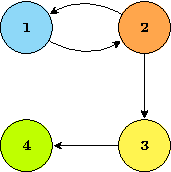
\includegraphics[height=0.2\textwidth]{Images/directed_graph}
    }
    %\quad
    \hspace{0.15\textwidth}
    \subfloat[Undirected Graph\label{fig:undirected_graph}]{
        \captionsetup{width=.4\textwidth}
        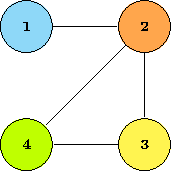
\includegraphics[height=0.2\textwidth]{Images/undirected_graph}
    }
    %\caption[Shorter caption]{This is a very long caption you don't want to appear in the List of Figures.}
    \caption{Example of directed and undirected graphs}
    \label{fig:directed_vs_undirected}
\end{figure}

Graphs serve as a versatile tool for describing diverse forms of data.
For example, molecules, the fundamental units of matter, are composed of atoms and electrons arranged in three-dimensional space.
In this intricate structure, all particles interact with each other.
However, when a pair of atoms are stably positioned at a specific distance, we refer to their connection as a covalent bond.
These bonds with distinct atomic distances can vary in nature, such as single or double bonds.
Representing this complex three-dimensional object as a graph offers a practical and widely adopted abstraction, where atoms are nodes and covalent bonds act as edges~\cite{DBLP:journals/corr/DuvenaudMAGHAA15}.

Social networks provide another domain where graphs are used: in fact, they serve as valuable tools for examining patterns within the collective behavior of people, institutions, and organizations.
By representing individuals as nodes and their relationships as edges, we can construct a graph that effectively captures groups of people and their interconnectedness.

\subsection{Graph Representation}
\label{subsec:graph_representation}

Graphs are easy to visualize, but a more formal way is needed when implementing graph algorithms.

\textbf{Adjacency matrix} \newline
The adjacency matrix of a graph is a fundamental representation that provides information about the relationships between nodes in the graph.
It provides a compact and easily interpretable representation of the graph's edges and connections, which can be easily implemented in almost all programming languages using two-dimensional arrays.

The adjacency matrix of a graph is a matrix of dimensions $N \times N$ where $N$ is the number of nodes in the graph.
Each matrix cell is set to 1 if the two nodes are connected, i.e.\ if there is an edge starting from the node of the corresponding row to the one of the corresponding column, and zero otherwise.
If the graph is undirected, each edge is bidirectional and so the matrix is symmetric.
If in the graph there are no self-loops, then the main diagonal of the matrix will be with all zeros.
Figure~\ref{fig:graph_adjacency} shows a directed graph and its adjacency matrix.

\begin{figure}[t]
    \centering
    \subfloat[Graph\label{fig:graph_example}]{
        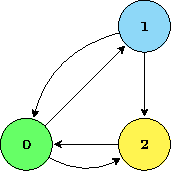
\includegraphics[height=0.2\textwidth]{Images/graph_example}
    }
    %\quad
    \hspace{0.15\textwidth}
    \subfloat[Adjacency matrix\label{fig:adjacency_mat}]{
        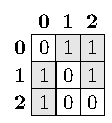
\includegraphics[height=0.2\textwidth]{Images/adjacency_matrix}
    }
    \caption{Example of a graph and its adjacency matrix}
    \label{fig:graph_adjacency}
\end{figure}

The adjacency matrix consists only of ones and zeros.
In real-world graph-related problems, the number of edges is usually much slower than the number of nodes, leading to an adjacency matrix with many zero elements.
Such matrices with mostly zero elements are called sparse matrices.
Their sparsity enables more efficient storage and manipulation, avoiding both the storage of zeros and the operations including zero elements, reducing the computational phase.

There are two common representations for sparse matrices: the Coordinate List (COO) format and the Compressed Sparse Row (CSR) format, which are explained below.

\begin{figure}[t]
    \centering
    \subfloat[COO format\label{fig:coo}]{
        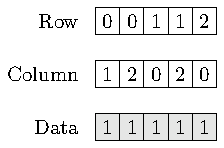
\includegraphics[height=0.2\textwidth]{Images/coo}
    }
    %\quad
    \hspace{0.15\textwidth}
    \subfloat[CSR format\label{fig:csr}]{
        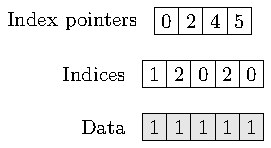
\includegraphics[height=0.2\textwidth]{Images/csr}
    }
    \caption{COO and CSR format of Adjacency matrix in Figure~\ref{fig:graph_adjacency}}
    \label{fig:coo_csr}
\end{figure}

\textbf{Coordinate format} \newline
In the COO format, a sparse matrix is represented as a list of [row, column, data] tuples, where each tuple corresponds to a non-zero element in the matrix.
The [row, column] coordinates represent the position of the non-zero element, and the value is the actual numerical value of that element.
Usually, it is preferred to store the entries first by row index and then by column index, to improve random access times.
In Figure~\ref{fig:coo_csr} the COO format of the adjacency matrix represented in Figure~\ref{fig:graph_adjacency} is reported.
For example, by considering the first element of the three arrays, it is possible to understand that the data one is placed in position [0, 1] of the adjacency matrix.

The COO format is helpful for matrices with relatively few non-zero elements because it does not require any assumptions about the sparsity pattern and allows for efficient deletion and insertion of elements.
However, it may not be the most efficient format for large and highly sparse matrices, as it may require more memory and may not support efficient row-wise or column-wise operations.
In these cases, other formats, like the CSR one, are often preferred.

\textbf{Compressed Sparse Row format} \newline
In the CSR format, a sparse matrix is represented using three arrays: the values array, the row pointers array (indices), and the column indices array (index pointers).
The data array contains the non-zero elements of the sparse matrix stored in row-major order, the array indices contains the column position of each data, while the index pointers
contains an increasing number of how many non-zero elements there are in the matrix row by row.
Given a matrix of size $m \times n$, with $NNZ$ being the number of non-zero elements, the arrays data and indices are of length $NNZ$, while the array index pointers is of length $m+1$.
Figure~\ref{fig:csr} shows the CSR format of the adjacency matrix represented in Figure~\ref{fig:graph_adjacency} is reported.

\textbf{Feature matrix} \newline
Suppose to have a graph of a social network, where each node corresponds to a person and each edge to a friendship on the social media between the two nodes.
If the aim is to predict the possible future friendship that could be established, maybe putting those people in the suggested friend list, having more information (features) about each node, such as the age or the gender, is helpful.

A feature vector represents the features or attributes associated with a single entity.
The feature matrix of a graph contains multiple feature vectors; it represents the features or attributes associated with each node.
It is commonly denoted as $X$ and  each row corresponds to a node in the graph, and each column corresponds to a specific feature or attribute of that node.

\section{Graph Neural Networks}
\label{sec:graph_neural_networks}%

%TODO: add an example image of a GNN

Graph neural networks (GNNs) are deep learning techniques that operate on graph-structured data.
Thanks to their impressive performance, GNNs have recently gained significant popularity as a widely adopted method for graph analysis~\cite{KERAMATFAR2022100401}.
Figure~\ref{fig:google_scholar} illustrates the steady growth in the number of publications related to Graph Neural Networks (GNNs) on Google Scholar from 2015 to 2022.
The data were collected by querying papers containing the specific words "Graph Neural Network" in their whole content and aggregating them on a yearly basis.
The increasing trend reflects the rising interest and research activity in the field of GNNs over the years.

\begin{figure}[t]
    \centering
    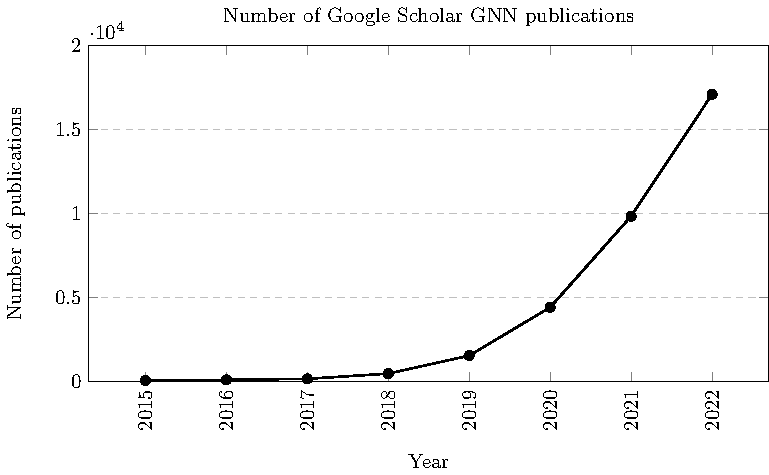
\includegraphics[height=0.4\textwidth]{Images/google_scholar}
    %\caption[Shorter caption]{This is a very long caption you don't want to appear in the List of Figures.}
    \caption{Number of GNN publications on Google Scholar per year}
    \label{fig:google_scholar}
\end{figure}

Graph Neural Networks are a group of neural networks which are designed to solve different tasks.
Prediction tasks on graphs can generally be classified into three categories: graph-level, node-level, and edge-level predictions~\cite{sanchez-lengeling2021a}.

In a graph-level task, the objective is to predict the property or characteristic of an entire graph.
For instance, when considering a molecule represented as a graph, attributes might be aimed to be predicted such as its likelihood of binding to a receptor associated with a specific disease.
This assignment is comparable to image classification tasks, where the objective is to assign a label to an entire image.
Similarly, in text analysis, sentiment analysis serves as a similar problem where the goal is to determine a complete sentence's overall mood or emotion in one go.

Node-level tasks involve predicting the identity or function of individual nodes within a graph.
One example of a node-level task is node classification in a social network.
Given a social network graph where nodes represent individuals and edges represent relationships between them, the task is to predict the demographic attributes or characteristics (e.g., age, gender, occupation) of each node based on their connection patterns and features.
Drawing an analogy to image processing, node-level prediction problems can be compared to image segmentation tasks, where the objective is to assign labels to each pixel in an image based on its role.
Similarly, in text analysis, a comparable task would involve predicting the parts of speech for each word in a sentence, such as identifying whether a word is a noun, verb, adverb, and so on.

The remaining prediction task in graphs pertains to edge prediction.
One example of an edge-level task is link prediction in a social network.
Given a graph representing a social network where, as before, in node-level tasks, nodes correspond to individuals and edges represent relationships between them, the edge-level task aims to predict missing or potential connections between nodes.
This can involve predicting the likelihood of a future friendship or the probability of a collaboration between individuals based on their shared characteristics or mutual connections in the network.

Graph Neural Networks (GNNs) are designed to process graph data and consist of multiple interconnected layers.
At its core, a GNN is an algorithm that exploits the connectivity within a graph to understand and represent the relationships between nodes.
By relying on the graph's structure, the GNN iteratively processes input edge, vertex, and graph feature vectors, which encode known attributes and transforms them into output feature vectors that capture the desired predictions.
Each Graph Neural Network typically encompasses three main stages: pre-processing, iterative updates and decoding or readout~\cite{DBLP:journals/corr/abs-2010-00130}.
\begin{enumerate}
    \item \textbf{Pre-processing}: this initial step, while optional, involves transforming the input feature vectors and graph structure representation through a pre-processing procedure.
    \item \textbf{Iterative updates}: following pre-processing, the feature vectors of each edge and vertex undergo iterative updates using aggregate-combine functions.
          For edge updates, attributes from the edge itself, connected vertices, and the graph are aggregated and combined to generate a new edge feature vector.
          Similarly, vertex updates involve aggregating feature vectors from neighboring vertices $\mathcal{N}(v)$ and combining them to obtain a new feature vector.
          This iterative process gradually incorporates relationships between increasingly distant nodes and edges, allowing for multi-hop updates.
          Furthermore, the graph may coarsen through pooling~\cite{DBLP:journals/corr/abs-1806-08804} (i.e. selective reduction or adjustment of either the graph structure or the neighborhood set of each node) in each subsequent layer, or the neighborhood set may change via layer sampling~\cite{DBLP:journals/corr/HamiltonYL17} (i.e. coarsening the graph from one layer to the next, leading to a reduction in the number of nodes that need to be processed during aggregation and combination steps).
    \item \textbf{Decoding or readout}: once the graph possesses a global feature vector, it is updated once upon completion of edge and node updates.
          The final output can be an edge/node embedding, representing specific information about each edge or node in a low-dimensional feature vector format, or a graph embedding that summarizes the entire output graph.
\end{enumerate}
Performing these stages on large and sparse graphs can introduce dynamic computational data flow and numerous irregular memory access patterns.

GNNs, as previously said, are structured into layers, each representing an iteration in the update process described earlier.
This layering allows information to propagate across nodes, enabling the influence of distant nodes.
Consequently, the appropriate number of layers in a GNN will vary depending on the significance of relationships among distant nodes in a specific application.
The commonly adopted range for the number of GNN layers is 1 to 5, as an excessive number of layers can introduce undesired problems such as feature over-smoothing, vanishing gradients, or over-fitting~\cite{DBLP:journals/corr/abs-1801-07606}.

Different popular Graph Neural Network architectures have been proposed recently, some of which are more suitable for some tasks than others.
A summary of two types of GNNs is provided in the following subsections, preceded by an important definition.

\subsection{Multi-Layer Perceptron}
\label{subsec:mlp}%
The central component of an Artificial Neural Network is referred to as the Multi-Layer Perceptron (MLP).
As depicted in Figure~\ref{fig:mlp}, it comprises multiple interconnected layers, each containing processing elements (neurons) that perform weighted sums of inputs and biases.

Input layers receives the input data, where each neuron represents a feature or attribute.
Hidden layers are responsible for learning and extracting complex features from the input data.
Output layers generate the final output of the network.
Processing elements in each layer receive inputs from all nodes in the previous layer and send their outputs to all neurons in the subsequent layer.

\begin{figure}[t]
    \centering
    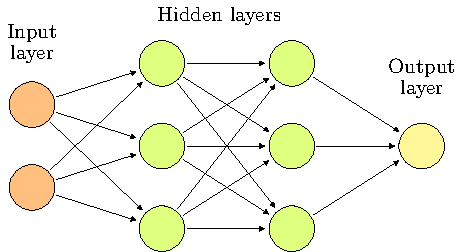
\includegraphics[height=0.3\textwidth]{Images/multi-layer-perceptron}
    \caption{Example of a Multi-Layer Perceptron}
    \label{fig:mlp}
\end{figure}

\subsection{Graph Convolutional Network}
\label{subsec:graph_convolutional_network}%

A graph convolutional network (GCN)~\cite{DBLP:journals/corr/KipfW16, daigavane2021understanding} is a type of neural network architecture explicitly designed to operate on graph-structured data.
GCNs aim to learn node representations by aggregating and combining information from neighboring nodes in the graph.
The core idea behind GCNs is to perform convolution-like operations on the graph, where the convolutional filters are defined based on the graph's adjacency matrix or other graph-specific structures.
This enables GCNs to capture and leverage the structural information encoded in the graph to make predictions or perform downstream tasks.
GCNs have demonstrated effectiveness in various applications, including node classification, link prediction, and graph classification.

Given an undirected graph $\mathcal{G} = (V, E)$, where $V$ represents the set of nodes (vertices), and $E$ represents the set of edges, with an adjacency matrix $\tilde{A}=A+I_N$, where $I_N$ is the identity matrix, the layer-wise propagation rule in a GCN can be expressed as:
\begin{equation}
    \label{eq:gcn_convolution}
    H^{(l+1)} = f \left( \tilde{D}^{-\tfrac{1}{2}}  \tilde{A}  \tilde{D}^{-\tfrac{1}{2}}  H^{(l)}  W^{(l)} \right)
\end{equation}

Where $H^{(l)} \in \mathbb{R}^{N \times D}$ is the input node features matrix, $W^{(l)}$ is a layer-specific learnable weight matrix, $\tilde{D}$ is the degree matrix defined as $\tilde{D}_{ii} = \sum_{j} \tilde{A}_{ij}$, and $f(\cdot)$ represents a non-linear activation function applied element-wise, such as $ReLU(\cdot) = max(0, \cdot)$.
The equation above demonstrates the propagation of node features through graph convolution, where the adjacency matrix $\tilde{A}$ captures the connectivity information of the graph, $\tilde{D}^{-\tfrac{1}{2}}$ normalizes the adjacency matrix, and $H^{(l)}  W^{(l)}$ performs a linear transformation of node features.
The resulting $H^{(l+1)}$ represents the updated node representations after the graph convolution operation.
In practice, multiple graph convolutional layers can be stacked to capture increasingly complex relationships and further refine the node representations.

\subsection{Graph Isomorphism Network}
\label{subsec:graph_isomorphism_network}%

A Graph Isomorphism Network (GIN)~\cite{xu2019powerful, daigavane2021understanding} is a type of neural network architecture designed to operate on graph-structured data by capturing graph isomorphism, which is the property of two graphs having the same structure, inspired by the Weisfeiler-Lehman (WL) graph isomorphism test~\cite{weisfeiler1968reduction}.
The WL test involves an iterative process where it (1) aggregates the labels of nodes and their neighborhoods, and (2) hashes the aggregated labels into unique new labels.
The algorithm determines that two graphs are non-isomorphic if, during any iteration, the labels of the nodes between the two graphs differ.
GINs aim to learn node representations that are invariant under graph isomorphism, enabling them to generalize across different graphs with similar structures.

The learned vertex features from GIN-Conv can be directly utilized for tasks such as node classification and link prediction.
The model is based on the following rule:
\begin{equation}
    \label{eq:gin_function}
    h_v^{(k+1)} = MLP^{(k)} \left( \left( 1 + \epsilon^{(k)} \right) \cdot h_v^{(k)} + \sum_{u \in \mathcal{N}(v)} h_u^{(k)} \right)
\end{equation}

Where $h_v^{(k)}$ represents the initial node representation of node $v$, $\mathcal{N}(v)$ represents the neighborhood of node $v$, $\epsilon$ is a learnable
parameter or a fixed scalar, $MLP( \cdot )$ represents a Multi-Layer Perceptron, defined in Subsection~\ref{subsec:mlp}, and $h_v^{(k+1)}$ represents the updated node representations.

In the neighborhood aggregation process of GINs, each node's representation is updated by considering its own representation and its neighbors' representations.
The neighborhood aggregation is performed through the MLP operation, followed by non-linear activation.

GINs are trained using graph-level objectives, such as graph classification or property prediction, and aim to learn invariant representations under graph isomorphism, allowing them to generalize well to unseen graphs with similar structures.
However, even if the node embeddings acquired through GIN can be directly applied to tasks such as node classification and link prediction, in the case of graph classification tasks, it is necessary to use a Readout function that takes individual node embeddings as input and produces the embedding representation for the entire graph.

The Readout function is then utilized to generate the overall representation of the graph, leveraging the individual vertex representations.
By concatenating the results from all iterations of GINConv, the final graph representation is obtained as:
\begin{equation}
    \label{eq:gin_readout}
    h_G = CONCAT \left( READOUT \left( \left\{ h_v^{(k)} | v \in G \right\} \right) | k = 0, 1, ..., K \right)
\end{equation}

Where $READOUT$ in~\ref{eq:gin_function} can be replaced with a sum operator in order to generalize the WL test.

\section{MLIR}
\label{sec:mlir}%
MLIR~\cite{9370308} represents a novel approach for constructing reusable and extensible compiler infrastructure.
Addressing software fragmentation and enabling compilation for heterogeneous hardware reduces the effort to build domain-specific compilers and seamlessly connect existing compilers.
MLIR empowers the design and implementation of code generators, translators, and optimizers across various levels of abstraction, application domains, hardware targets, and execution environments.

The MLIR project aims to address programming language design and implementation challenges.
It achieves this by enabling cost-effective definition, introducing new abstraction levels, and built-in infrastructure to solve common compiler engineering issues.
MLIR ensures extensibility through Dialects, which logically group Ops, attributes, and types under a unique namespace.
Dialects do not introduce new semantics but act as a mechanism for group-related functionality, such as constant folding behavior, for all ops in the dialect.
They organize the ecosystem of language- and domain-specific semantics while adhering to the principle of simplicity.
Unknown Ops are treated with a conservative approach by compiler passes, and MLIR offers extensive support for describing the semantics of Ops to passes through traits and interfaces.

\section{High-Level Synthesis}
\label{sec:hls}%

This thesis presents a toolchain leveraging High-Level Synthesis (HLS) to automatically translate algorithmic descriptions of applications into low-level RTL (register-transfer level) descriptions or digital circuits.
HLS tools simplify hardware development's most complex and time-consuming aspect by allowing users to provide programs written in common programming languages like C/C++, eliminating the need for manual VHDL/Verilog coding.
HLS significantly reduces design time and effort, making the final implementation's functionality independent of hardware design knowledge.

The High-Level Synthesis process~\cite{5209958}, depicted in Figure~\ref{fig:hls}, begins with compiling the functional specification, transforming it into a formal representation, and applying various code optimizations.
The allocation phase determines the type and quantity of hardware resources required to meet design constraints.
In the scheduling phase, all operations within the specification model are scheduled into cycles.
The operation's scheduling can vary based on the functional component to which it is mapped, resulting in either single-clock-cycle scheduling or multi-cycle scheduling.
The binding algorithm optimizes the selection of storage units for variables carrying values across cycles and the assignment of functional units for each operation in the specification model.
The next step is to generate an RTL model of the synthesized design, incorporating all the design decisions made.

\begin{figure}[t]
    \centering
    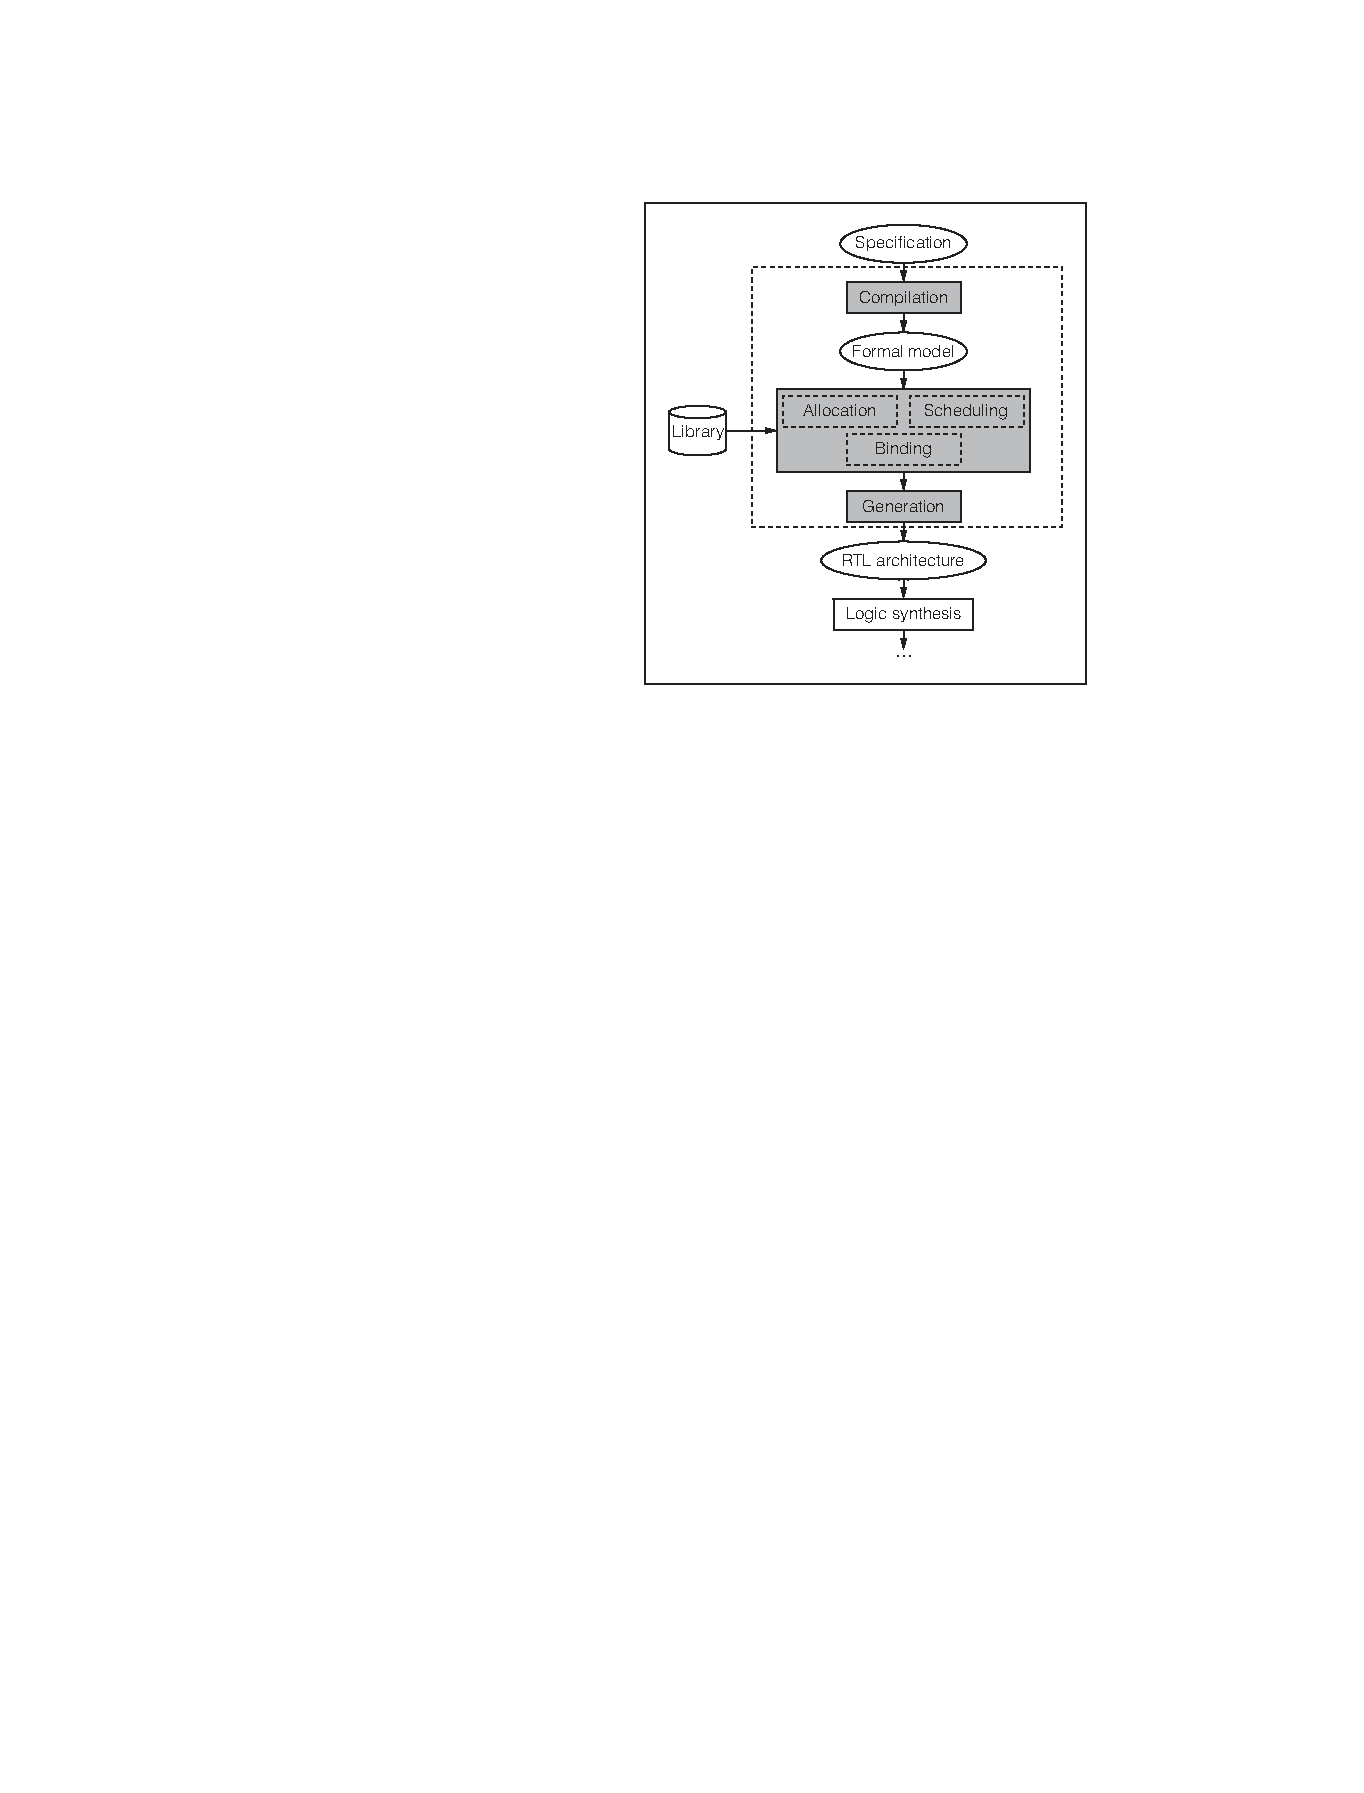
\includegraphics[height=0.4\textwidth]{Images/hls}
    \caption{High-level Synthesis (HLS) design steps~\cite{5209958}}
    \label{fig:hls}
\end{figure}

\section{LLVM}
\label{sec:llvm}%

LLVM is a compiler framework that enables ongoing analysis and transformation of programs through a code representation independent of any specific language.

Many HLS frameworks rely on it, thanks to its intermediate level of abstraction.
It is also the case of the HLS tool used for this thesis, which takes an LLVM representation as input.

The LLVM Intermediate Representation (IR), which resembles the assembly code, is a low-level code representation.
LLVM uses a language-independent type system and utilizes an infinite set of virtual registers.
All instructions follow the Static Single Assignment (SSA) form, meaning each virtual register appears in only one instruction, and each instruction takes one or two input operands while producing a single result.

\section{SODA Toolchain}
\label{sec:soda}%

SODA~\cite{9786533} is a software-defined accelerator synthesizer.
It enables the creation of highly specialized accelerators from algorithms designed in high-level programming frameworks.
The synthesizer comprises a compiler-based frontend that interfaces with high-level programming frameworks, applying advanced optimizations.
It also includes a compiler-based backend responsible for generating Verilog code and interfacing with external tools to compile the final design, which can be applied to application-specific integrated circuits (ASICs) or field-programmable gate arrays (FPGAs).

SODA's exceptional power lies in its ability to offer a fully automated end-to-end hardware compiler, eliminating the need for human intervention and any modifications to the input code.
This framework seamlessly integrates with high-level Python frameworks by accepting their input descriptions, which are then translated by the frontend into a high-level intermediate representation (IR).
Leveraging the multi-level intermediate representation (MLIR), the frontend facilitates hardware/software partitioning of algorithm specifications and performs architecture-independent optimizations.
Following this, it generates a low-level IR (LLVM IR) that is utilized by the hardware generation engine, PandA-Bambu~\cite{9586110}.
PandA-Bambu can accept LLVM IR as input, making it a cutting-edge open-source HLS tool.
Throughout the entire SODA toolchain, compiler passes are employed to implement optimizations at all levels, greatly influencing the generated hardware designs' performance, area, and power characteristics.

\subsection{SODA-OPT Frontend}
\label{subsec:soda_frontend}%

SODA-OPT, the high-level compiler frontend of the SODA synthesizer, performs search, outlining, optimization, dispatching, and acceleration passes on the input program.
Its primary objective is to prepare the program for hardware synthesis, targeting either FPGAs or ASICs.
To accomplish these tasks, SODA-OPT relies on and extends the MLIR framework.
MLIR is a framework that facilitates the development of reusable, extensible, and modular compiler infrastructure by defining dialects.
These dialects serve as self-contained intermediate representations (IRs) that adhere to the meta-IR syntax of MLIR.
By utilizing dialects, code can be modeled at different levels of abstraction, allowing for specialized representations that aid in specific compiler optimizations.

 Code regions selected for hardware acceleration undergo an optimization pipeline that progressively lowers them through various MLIR dialects until they are ultimately translated into an LLVM IR format tailored explicitly for hardware synthesis.
On the other hand, the host module is lowered into an LLVM IR file containing runtime calls to control the generated custom accelerators.

\subsection{SODA Synthesizer Backend}
\label{subsec:soda_backend}%

Bambu, the SODA synthesizer backend, harnesses cutting-edge HLS techniques to produce accelerator designs using the low-level LLVM IR generated by the SODA frontend.
Bambu supports multiple frontends based on standard compilers such as GCC or CLANG.
It constructs an internal IR to execute HLS steps and generates designs in HDL formats, such as Verilog or VHDL.
In addition to synthesizable HDL, Bambu can automatically generate testbenches for verification purposes.
Using Bambu, the SODA synthesizer can target both FPGAs and ASICs.

Bambu is optimized to handle a broad range of C and C++ constructs while also being able to process LLVM IR through its internal Clang frontend.
Through SODA-OPT, Bambu can be connected with MLIR code.
The LLVM IR generated after SODA-OPT's high-level optimizations undergoes explicit restructuring for HLS, resulting in more efficient accelerators than direct translation from MLIR to LLVM IR.

\section{Conclusion}
\label{sec:background_conclusion}%
This chapter has presented the foundational concepts necessary for understanding the subsequent contents of this thesis.
It provided a concise overview of the broad domain of Graphs and Graph Neural Networks, explicitly focusing on the architectures of Graph Convolutional Networks and Graph Isomorphism Networks.
Additionally, the chapter introduced SODA and PandA-Bambu, which will be further investigated within the context of the proposed design flow for the creation of GNNs FPGA-based accelerators.

The following chapter is dedicated to an analysis of scientific literature on hardware acceleration for Graph Neural Networks.
This analysis primarily focuses on publications concerning FPGA-based implementations and design flows that leverage High-Level Synthesis techniques.


% ##########################################################################
% CHAPTER THREE - RELATED WORK
% ##########################################################################


    \chapter{Related Work}
    \label{ch:chapter_three}%
    Accelerating Graph Neural Networks (GNNs) has become a subject of intense interest within the research community, encompassing the exploration of ASIC and FPGA accelerators.
In this chapter, a comprehensive examination is conducted on cutting-edge Graph Neural Networks FPGA accelerators and design flows based on High-Level Synthesis (HLS).
As explained in Chapter 6, particular emphasis has been placed on optimizing matrix-matrix multiplication during this thesis research study.
Consequently, this chapter also delves into the relevant literature concerning various approaches to Matmul optimization.

\section{Chapter structure}
\label{sec:related_work_structure}%
This chapter contains several sections.
Firstly, it presents the software frameworks utilized to accelerate Graph Neural Network computations.
The following section provides an overview of state-of-the-art hardware accelerators, categorized based on their architecture types~\cite{DBLP:journals/corr/abs-2010-00130}.

Subsequently, a section summarizes an accelerator implemented using High-Level Synthesis (HLS). This accelerator is separated from the hardware accelerators as it adopts HLS as the design flow proposed in this thesis.

Additionally, this chapter includes a summary of a solution that aimed to accelerate GNN using both software and hardware approaches.
A section is dedicated to a state-of-the-art graph processing accelerator, implemented using HBM-equipped FPGAs.

As mentioned earlier, optimizing the matrix-matrix multiplication operation was a significant aspect of this research.
Thus, a dedicated section focuses on state-of-the-art optimizations for matrix-matrix multiplication, especially those related to technologies similar to the ones employed in this thesis.

Finally, the chapter concludes with a comprehensive summary of the cutting-edge accelerators presented.

\section{Software accelerators}
\label{sec:related_work_software_accelerators}%

The challenges posed by GNN processing have led to inefficiencies in traditional deep neural network (DNN) libraries and graph processing frameworks.
This is primarily due to the alternating computational phases characteristic of GNNs.
While DNN libraries excel in accelerating combination operations within vertices and edges, they need help with aggregation tasks.
On the other hand, graph processing libraries effectively handle irregular memory accesses during graph traversal but assume simplistic operations at the vertices, which is not the case in GNNs. Recent research studies tried to bridge the gap by adapting the DNN libraries to overcome Graph Neural Network challenges.

The two main software frameworks trying to accelerate Graph Neural Networks computation are PyTorch Geometric~\cite{DBLP:journals/corr/abs-1903-02428} and Deep Graph Library~\cite{DBLP:journals/corr/abs-1909-01315}.
They both provide a lot of examples and code for multiple GNN architectures providing optimizations that could work for the acceleration of both training and inference.

PyTorch Geometric is a PyTorch-based library specifically designed for deep learning on input data with irregular structures, including graphs, point clouds, and manifolds.
In addition to offering comprehensive graph data structures and processing techniques, it incorporates many state-of-the-art methods from relational learning and 3D data processing domains.
PyTorch Geometric achieves remarkable data throughput by introducing efficient handling of mini-batches containing input examples of varying sizes and efficiently handling sparsity through specialized GPU scatter and gather kernels, which operate on all edges and nodes concurrently, as opposed to relying on sparse matrix multiplication kernels.
A key aspect of PyG involves defining a message-passing interface encompassing message and update functions for neighborhood aggregation and combination and multiple pooling operations.

DGL is a recently developed library that seamlessly integrates with TensorFlow, PyTorch, or MXNet.
It introduces three essential functions: message for aggregating edges, update and reduce for aggregating and combining at the nodes.
DGL adopts a matrix multiplication approach to enhance performance and harnesses specialized kernels designed for GPUs or TPUs.
Specifically, both sampled dense-dense and sparse matrix multiplications and options for node, edge, or feature parallelization are considered.
DGL intelligently selects the optimal parallelization scheme using heuristics, considering various factors, including the input graph.
It distills the computational patterns of GNNs into a set of generalized sparse tensor operations, which facilitate extensive parallelization.
By prioritizing the graph as the central programming abstraction, DGL enables transparent optimizations.
Furthermore, through a framework-neutral design philosophy, DGL allows users to effortlessly port and leverage existing components across multiple deep learning frameworks.

The approach used by DGL outperformed PyTorch Geometric in training Graph Neural Networks, as stated in their paper~\cite{DBLP:journals/corr/abs-1909-01315}.
However, both libraries target CPU and GPU architectures.
Knowing the extreme computational power of FPGA, the field of hardware accelerators started gaining more and more interest, with the expectation of having GNN hardware accelerators capable of outperforming the performance of CPU-GPU targeting libraries.

\section{Hardware accelerators}
\label{sec:hardware_accelerators}%

As discussed in Section~\ref{sec:related_work_software_accelerators}, software accelerators optimize the execution of GNNs in CPU-GPU platforms, commonly found in various computing systems, leading to substantial speed improvements in inference and training processes.

However, the research field has raised questions about the feasibility of custom hardware accelerators in overcoming the challenges of GNN computing and achieving order-of-magnitude enhancements.
Consequently, numerous hardware accelerators with different architecture types have emerged, aiming to address the intensive computational demands and alternating patterns required by GNNs.

\subsection{Unified architecture accelerators}\label{subsec:unified-architecture-accelerators}%

A unified architecture refers to a design approach where the FPGA fabric is configured to be versatile and flexible, allowing it to handle various applications and tasks.
Instead of having specialized and fixed hardware modules for specific functions, a unified architecture enables the FPGA to reconfigure its resources to dynamically adapt to different computation requirements.

\cite{DBLP:journals/corr/abs-1908-10834} presents Autotuning-Workload-Balancing GCN (AWB-GCN) to accelerate Graph Convolutional Network inference.
This accelerator endorses a proactive adaptation to the structural sparsity inherent in GNNs. The authors support their design by analyzing the power-law distribution found in most graphs, positing that certain parts of the computation will exhibit density. In contrast, others will be extraordinarily sparse, leading to imbalances.

In order to tackle this problem, the architecture devises a custom matrix multiplication engine that efficiently supports skipping zeros.
In particular, three hardware-based autotuning techniques to address the imbalance have been suggested: dynamic distribution smoothing, remote switching, and row remapping.

Specifically, AWB-GCN continuously monitors the sparse graph pattern, dynamically adjusts the workload distribution among many processing elements, and reuses the optimal configuration upon convergence.
Data from memory is directed through a task distributor and queue (TDQ) to a collection of processing elements (PEs) and accumulators.
The TDQ has two designs tailored for scenarios with moderate or high sparsity.
Given AWB-GCN's emphasis on GCNs featuring linear aggregation functions, the authors suggest prioritizing combination processing, as this typically reduces the number of features and subsequently minimizes the operations performed during aggregation.
Additionally, AWB-GCN incorporates a fine-grained pipelining mechanism to effectively overlap the execution of combination and aggregation, even within the same layer.

However, at the heart of the AWB-GCN architecture lies the management of load balancing at three levels of granularity: distribution smoothing to handle local utilization fluctuations among PEs, remote switching for minor crests, and row remapping for prominent crests.
At the beginning of the processing, rows are evenly distributed among processing elements.
Throughout each round of calculation, distribution smoothing equalizes the workloads among neighboring PEs.
The architecture of AWB-GCN effectively monitors the runtime PE utilization by tracking the number of pending tasks in task queues.
It continually offloads the work from more burdened PEs to their less occupied neighbors, up to 3-hop neighbors.

Remote switching is implemented to tackle regional clustering, wherein the process facilitates partial or complete workload exchanges between underutilized and overloaded PEs.
An auto-tuner dynamically determines the switch fraction at runtime, relying on the PE utilization observed in each round.
The accelerator retains the switch strategies employed in the current round and iteratively optimizes them based on utilization information gathered in the subsequent round.
As a result, after several rounds of auto-tuning, the switch strategy that best aligns with the sparse matrix structure is attained and is then utilized for the remaining rounds, leading to nearly perfect PE utilization.

Lastly, the evil-row remapping technique redistributes the evil row to the most under-loaded PEs in troughs, allowing the neighboring PEs to assist.
Row remapping is initiated based on demand after each round.
The auto-tuner assesses the utilization gaps between the most overloaded and under-loaded PEs and decides if their gaps exceed remote switching capability.
If so, row remapping is executed as a solution.

AWB-GCN proves to be a fascinating accelerator, though its generalizability beyond Graph Convolutional Network remains uncertain.
On the other hand, EnGN represents another accelerator featuring a unified architecture, with the primary goal of being adaptable for various Graph Neural Network models.

EnGN~\cite{DBLP:journals/corr/abs-1909-00155} is a specialized accelerator architecture that prioritizes high-throughput and energy-efficient processing of large-scale GNNs in which the Graph Neural Network is treated as a concatenated matrix multiplication of feature vectors, adjacency matrices, and weights, all efficiently scheduled in a single data flow.
An array of clustered Processing Elements (PEs) is supplied with independent banks for features, edges, and weights, enabling computation of the combination function.

EnGN accelerates the three fundamental stages of GNN propagation to handle sparsity efficiently, i.e., feature extraction, aggregate, and update, which encapsulates common computing patterns shared by typical GNNs.
The authors introduce the ring-edge-reduce (RER) dataflow for the aggregation, in which each column of PEs is interconnected through a ring, and results are passed along and added based on the adjacency matrix.
This process effectively addresses the poor locality of sparsely and randomly connected vertices and efficiently supports critical stages. EnGN dynamically reorders edges in each RER step to reduce redundant computations in sparsely connected nodes.

Moreover, EnGN employs a graph tiling strategy to accommodate large graphs, optimizing the utilization of hierarchical on-chip buffers through adaptive computation reordering and tile scheduling.
This approach enhances EnGN's capability to handle substantial graphs effectively.

Since well-connected vertices frequently appear during computation, PE clusters have a degree-aware vertex cache that stores data for high-degree vertices.
Other optimized design decisions in EnGN involve the order of matrix multiplications when the aggregation function is a sum, impacting the total number of operations.

Moreover, EnGN employs a graph tiling strategy to accommodate large graphs, optimizing the utilization of hierarchical on-chip buffers through adaptive computation reordering and tile scheduling.
These optimizations collectively enhance the overall performance of EnGN for large-scale GNN processing tasks.

\subsection{GNN acceleration using Tiled architecture}
\label{subsec:tiled-architectures}%

A tiled architecture refers to a design approach where the FPGA fabric is organized into a regular grid-like pattern of configurable tiles.
Each tile typically consists of a set of logic cells, interconnect resources, and other functional units, and these tiles are repeated across the entire FPGA.

In contrast to most other accelerators, this work~\cite{9218751} presents a modular architecture for convolutional GNNs incorporating dedicated hardware units to efficiently handle the irregular data movement essential for graph computation in GNNs, while simultaneously delivering the high compute throughput required by GNN models.
The fundamental building block of the accelerator is a tile consisting of an aggregator module (AGG), a DNN accelerator module (DNA), a DNN queue (DNQ), and a graph PE (GPE), all interconnected via an on-chip router.

The Graph Processing Element (GPE) handles graph traversal and sequencing computation steps dependent on the underlying graph structure.
The DNA executes the DNN computation within the GNN model.
The AGG performs feature aggregation coordinated by the GPE based on graph traversal.
The DNQ buffers memory requests and intermediate results as they are passed to the DNA.

This design allows for easy scalability by interconnecting multiple tiles with memory.
Each tile's internal structure resembles HyGCN's~\cite{DBLP:journals/corr/abs-2010-00130}, with the DNA functioning as an array for dense multiplication, the AGG as an edge-controlled adder, the DNQ as an inter-engine buffer, and the GPE overseeing execution.

The GNN accelerator program proposed by Auten \textit{et al.} represents a GNN model as a sequential set of layers.
Each layer operates on a graph, applying a vertex program to generate an output graph.
These layers are connected in sequence to form a complete GNN model.
The initial layer takes the model input as its input graph, and subsequent layers utilize the output of the preceding layer.
The last layer produces the final output graph.

Unlike HyGCN, the accelerator introduced in~\cite{9218751} is less specialized but has a better potential for generalization to various Graph Neural Network models~\cite{DBLP:journals/corr/abs-2010-00130}.

\subsection{Hybrid architectures for GNN acceleration}
\label{subsec:hybrid-architectures}%

HyGCN~\cite{DBLP:journals/corr/abs-2001-02514} is a unique GCN accelerator due to its innovative hybrid architecture.
This approach was inspired by the observation that GNNs exhibit two distinct execution patterns with contrasting requirements: the aggregation phase involves graph processing, displaying a dynamic and irregular execution pattern.
On the other hand, the combination phase behaves more like conventional neural networks, exhibiting a static and regular execution pattern.
As a result of this observation, HyGCN consists of dedicated engines for the aggregation and combination stages and a coordinating mechanism for pipelined execution of both functions.

The Combination operation at each vertex functions like a neural network with a regular yet compute-intensive execution.
HyGCN's architecture is based on the popular systolic array, but it incorporates multiple arrays instead of a single one to adapt to the two processing modes of the Aggregation Engine.
In the combination engine, a set of systolic arrays is combined to form a systolic module, and these modules can be flexibly utilized in various ways, including independent and cooperative working modes.

\begin{itemize}
    \item In the independent working mode, the systolic modules operate autonomously, each handling the matrix-vector multiplication (MVM) operations of a small group of vertices.
          This mode offers the benefit of reduced vertex latency since the Combination operations for this smaller group of vertices can be processed immediately once their aggregated features are ready without waiting for additional vertices.
    \item In the cooperative working mode, a large group of vertices' aggregated features are gathered and combined.
          The advantage of this mode is that weight parameters can be efficiently reused by all systolic arrays, reducing energy consumption.
\end{itemize}

The aggregation engine comprises a sampler, edge scheduler, and sparsity eliminator feeding a set of SIMD (single instruction multiple data) cores.
There are two processing modes for SIMD cores to handle edges in parallel.

The first mode is vertex-concentrated, where each SIMD core is assigned the workload of a single vertex.
While this mode can produce aggregated features in a burst mode, the processing latency for a single vertex is prolonged, leading to workload imbalance and loss of parallelism.
On the other hand, the vertex-disperse processing mode assigns the aggregation of elements in the vertex feature vector to all cores.
This mode ensures that all cores are constantly busy without workload imbalance.
Additionally, it enables immediate processing of each vertex in the subsequent Combination Engine while reducing the latency for a single vertex compared to processing multiple vertices together.
To enhance the computation of aggregation, HyGCN uses the vertex-disperse processing mode.

HyGCN utilizes a static graph partition method to optimize memory access to improve data reuse.
The authors identified that the feature vectors of each vertex are typically large, making the exploitation of feature locality crucial.
To address this, they grouped vertices within the same interval and processed the aggregation of their source neighbors interval by the interval.
By following this approach, the feature accesses of all vertices in an interval were merged.
This grouping allowed for overlapping neighbors within the considered interval, enabling the reuse of loaded feature data during feature aggregation.
Moreover, when traversing all the neighbors of the interval, the intermediate aggregated results of the grouped vertices were stored in a buffer and could be reused during feature updates.

Sparsity is efficiently handled at the aggregation engine through effective scheduling and the sparsity eliminator, which adapts dynamically to varying degrees of sparse multiplications using a window-based sliding and shrinking approach.
In particular, the authors implemented this approach to enhance data reuse and minimize redundant accesses caused by sparse graph connections.
The central idea was to slide the window downward until an edge appeared in the top row and then shrink its size by moving the bottom row upward until an edge was encountered.
This method effectively eliminated sparsity and improved data access efficiency.

To further optimize for varying workloads, HyGCN allows flexible grouping of SIMD cores in aggregation and PEs in combination based on the size of feature vectors.
Additionally, careful attention is given to the design of the inter-engine coordinator to optimize memory accesses and enable fine-grained pipelining of execution, maximizing parallelism dynamically.

While not an authentic hybrid architecture, GRIP~\cite{DBLP:journals/corr/abs-2007-13828} is an accelerator that shares similar techniques with HyGCN's implementation approach.
It leverages GReTA~\cite{greta-recoml20} (Gather, Reduce, Transform, Activate), a graph processing abstraction specifically crafted for efficient execution on accelerators.
It also offers the flexibility required to implement GNN inference and holds the potential to be adaptable to various types of Graph Neural Networks.

GRIP is an accelerator designed to achieve low-latency inference.
It addresses the challenges of accelerating GNNs, combining two distinct computation types: arithmetic-intensive vertex-centric operations and memory-intensive edge-centric operations.
To tackle this, the accelerator divides GNN inference into fixed sets of edge- and vertex-centric execution phases, making them suitable for hardware implementation.
Each unit is then specialized to handle the unique computational structure of each phase efficiently.

GRIP utilizes a high-performance matrix multiply engine and a dedicated memory subsystem for vertex-centric phases for weights to enhance data reuse.
In contrast, it employs multiple parallel prefetches and reduction engines for edge-centric phases to mitigate the irregularity in memory accesses.
Additionally, GRIP supports several GNN optimizations, including a novel technique called vertex-tiling, which enhances the reuse of weight data.

GRIP provides a customizable architecture with separated and custom units and accumulators for both edges (gather, reduce) and vertices (transform, activate) that allows for performing edge and node updates using user-defined functions.
The control of GRIP is managed by a host system that issues commands for different operations and data transfers.
The control unit dequeues these commands in order and asynchronously issues them to individual execution units or the memory controller.

GRIP comprises three core execution units: the edge unit, the vertex unit, and the update unit.
The edge unit performs the edge-accumulate phase, iterating over the edges of the nodeflow, executing gather, and accumulating the result into the edge accumulator using reduce.
The vertex unit performs the vertex-accumulate phase, iterating over the output vertices corresponding to the accumulated edge values, executing the transform, and accumulating the result into the vertex accumulator.
The update unit performs the vertex-update phase, reading the accumulated values for each vertex and passing them to the activated PE.
The result is then written to the nodeflow buffer as an updated feature or to the edge or vertex accumulator, enabling efficient data flow between different GRIP programs when executed in sequence.

As already said, GRIP allows users to customize the four PEs, which can be implemented in multiple ways based on their specific requirements.
In the authors' implementation, a programmable ALU-based approach is used, splitting the edge update unit into lanes to execute vertices simultaneously.
It adopts an input-stationary dataflow for the vertex update unit.
The accelerator employs various optimizations, including pipelining and tiling adapted to the specific dataflows implemented, similar to other accelerators.

\section{High-Level Synthesis based accelerators}
\label{sec:hls-accelerators}%

As previously highlighted, the main challenge of GNN hardware acceleration lies in simultaneously meeting the demand for novel GNN models and fast inference, as there exists a gap between the difficulty in developing efficient FPGA accelerators and the rapid pace of creating new GNN models.

To address this challenge, in~\cite{DBLP:journals/corr/abs-2201-08475} GenGNN has been introduced, a GNN acceleration framework utilizing High-Level Synthesis (HLS), with two primary objectives.
Firstly, to achieve ultra-fast GNN inference without needing graph pre-processing to meet real-time demands.
Secondly, to support a wide range of GNN models with the flexibility to accommodate new models.
The framework incorporates an optimized message-passing structure that applies to all models and is complemented by a diverse library of model-specific components.

This framework capitalizes on the observation that each node in a GNN layer undergoes two key steps: message passing (MP) and node embedding (NE). The message passing step is further divided into gather and scatter phases, where gather involves feature aggregation, and scatter entails message transformation and forwarding.
On the other hand, node embedding encompasses node transformation and update.

To achieve this goal, GenGNN was designed using a message-passing style featuring two main processing elements (PEs): node embedding and message passing.
The architecture includes three data storage buffers: one node embedding buffer and two message buffers, all of which have a $O(N)$ size, where $N$ represents the number of nodes allowed on-chip.
The two message buffers are used alternately across layers, allowing for the reuse of resources and dataflow in multiple layers.
The node embedding PE handles node transformation and update within a single layer, while the message passing PE performs the subsequent scatter operation.
The advantage of this approach is that the receivers of the messages can instantly update their partially aggregated message in the message buffer, enabling the merging of scatter and gather phases.
Since the aggregation function is permutation invariant and the aggregation order does not matter, such a merged fashion reduces the overall process latency and minimizes memory cost.

The independence of node embedding (NE) and message passing (MP) steps across nodes and edges allows for significantly reduced processing latency by effectively pipelining these two steps.
The authors referred to the most suitable approach for this task as streaming-based pipelining, which can be achieved using a streaming-based FIFO (first-in-first-out) memory queue.
In this implementation that significantly reduces idle cycles and minimizes resource usage, NE and MP are pipelined flexibly using a node queue.
Once a node completes its NE and is prepared for message passing, its embeddings are pushed into the queue.
At the same time, the MP engine reads from the queue, fetching the node embeddings for message passing.

GenGNN enhances its architecture's adaptability to different graph neural network models by offering various model-specific components.
One particularly advantageous feature of GenGNN's streaming-based pipelining for node/edge processing is its suitability for models with virtual nodes.
As defined by~\cite{DBLP:journals/corr/GilmerSRVD17}, a virtual node acts as an artificial node connected to all other nodes in the graph, creating a shortcut for message passing between node pairs.
The authors stated that processing the virtual node can be entirely overlapped with the node embedding computation for other nodes, ensuring zero waste as long as it is handled early enough in the processing pipeline.

Finally, another feature provided by GenGNN is the large graph extension.
The authors implemented a prefetcher to accommodate large graphs that cannot be stored on-chip.
This prefetcher retrieves consecutive nodes' degrees from DRAM and stores them in an on-chip FIFO buffer.
As the message passing PE requires, it loads each subsequent node's degree, prompting the prefetcher to refill the buffer.
This clever mechanism effectively conceals the latency associated with fetching from the off-chip degree table, ensuring that the message passing PE behaves similarly to handling small graphs.
Moreover, the authors adopted packed data transfer by typecasting off-chip array pointers into the desired size pointer types, facilitating the transfer of more significant bits between DRAM and the system with every clock cycle.

It can be observed that GenGNN's NE/MP pipeline shares a similar concept with the task scheduling approach of BoostGCN~\cite{9444065}.

BoostGCN presents a framework tailored to enhance GCN inference on FPGA. The authors introduced a groundbreaking hardware-aware Partition-Centric Feature Aggregation (PCFA) scheme that capitalizes on 3-D partitioning alongside the vertex-centric computing paradigm.
This innovation significantly boosts on-chip data reuse while minimizing the overall data communication volume with external memory.

Furthermore, they devised a novel hardware architecture that enables seamless pipelined execution of the two distinct computation phases.
They developed a low-overhead task scheduling strategy to tackle any potential pipeline stalls arising from these phases.

The authors delivered a comprehensive GCN acceleration framework on FPGA, complete with meticulously optimized RTL (Register-Transfer Level) templates.
This framework can generate hardware designs based on personalized configurations and is adaptable to diverse GCN models.
BoostGCN's overall system architecture comprises external memory and FPGA components.
Feature Aggregation Modules (FAMs) handle feature aggregation on the FPGA board, while Feature Update Modules (FUMs) manage feature updates.
Intermediate results generated by FAMs are cached in the Internal Buffer, and the Memory Controller manages data transmissions between external memory and hardware modules.

The authors propose a specific approach to optimize task scheduling and minimize pipeline stalls for FUM and FAM. This involves arranging intervals based on their vertex degrees and prioritizing intervals with more minor vertex degrees for execution first.
Furthermore, they allocate a buffer in external memory to store aggregated feature vectors produced by FAMs in case FUM is not yet prepared to consume new aggregated feature vectors.
Subsequently, FUM can retrieve the aggregated feature vectors from external memory when ready.

As indicated in~\cite{DBLP:journals/corr/abs-2201-08475}, while the scheduling approaches of GenGNN and BoostGCN share some similarities, there are notable differences.
Firstly, BoostGCN relies on sorting vertices by degrees on the CPU to establish an execution order, whereas GenGNN processes the nodes on-the-fly in FPGA in an adaptive manner.
Secondly, BoostGCN employs a buffer in external memory, while GenGNN utilizes an on-chip FIFO to queue the nodes ready for message passing.

Another notable framework in this section is DGNN-Booster~\cite{chen2023dgnnbooster}, an innovative Field-Programmable Gate Array (FPGA) accelerator framework designed for real-time inference of Dynamic Graph Neural Networks (DGNNs) using High-Level Synthesis (HLS).
Unlike the other accelerators mentioned and outside the scope of this research, DGNN-Booster focuses on DGNNs, which are Graph Neural Networks tailored for dynamic graph structures and features.
Hence, a detailed description is not provided here.
However, it is worth mentioning that DGNN-Booster implements GNNs using a message-passing mechanism based on GenGNN at a lower level of parallelism.

\section{Software-Hardware co-design accelerators}
\label{sec:software-hardware-accelerators}%

The work conducted by Zhang \textit{et al.}~\cite{9153263} introduces a combined software and hardware approach for accelerating Graph Convolutional Networks (GCNs).
Their study was initiated with the recognition that hardware acceleration of Graph Convolutional Network (GCN) inference poses challenges stemming from the vast size of the input graph;
the heterogeneous workload of GCN inference involving sparse and dense matrix operations and the irregular information propagation along the edges during computation

The primary objective of this accelerator is to expedite GCN models, with a particular focus on accelerating the critical computational kernels: feature aggregation $AX$ and feature transformation $XW$.
In these kernels, $A$ represents the adjacency matrix, $X$ denotes the feature matrix, and $W$ represents the weight matrix.

The proposed algorithm-architecture co-optimization for accelerating large-scale Graph Convolutional Network (GCN) inference on FPGA involves several key steps.
First, the authors implemented a data partitioning scheme for GCN inference to accommodate real-world datasets with huge dimensions for $A$ and $X$.
This approach ensures that both the adjacency matrix and the feature matrix can fit on-chip while mapping the computational kernels onto the FPGA\@.

Then, the graph undergoes a two-phase preprocessing algorithm involving sparsification and node reordering. 
The sparsification phase eliminates edge connections of high-degree nodes by merging familiar neighbors to reduce the memory accesses that a graph with more edges can require during the aggregation stage.
The node reordering phase effectively groups adjacent nodes to enhance on-chip data reuse.

The pre-processed graph is then fed into a hardware accelerator implemented in an FPGA that efficiently pipelines GCN's two major computational kernels: aggregation and transformation.
As outlined in~\cite{DBLP:journals/corr/abs-2010-00130}, the design distinguishes itself from other approaches in several ways.
The aggregator module adopts a double-buffering technique to hide addition latency and leverages node- and feature-level parallelism.
Moreover, the accelerator supports two modes of operation depending on the order of matrix multiplications, leading to different pipelining strategies.
In order to accommodate these modes, the modules are interconnected from the aggregate module to the combination modules and vice versa.

GCoD~\cite{9773223} is another accelerator that follows the dedicated Algorithm and Accelerator Co-Design approach.
It is a framework combining Graph Convolutional Network algorithm and accelerator design to improve GCNs' inference efficiency significantly.

GCoD incorporates a split-and-conquer GCN training strategy at the algorithm level, dividing graphs into denser or sparser local neighborhoods without sacrificing model accuracy.
This approach leads to adjacency matrices with mainly two levels of workload, enabling more effortless acceleration.

GCoD's Split and Conquer Algorithm aims to tackle the high sparsity and irregularity in GCNs' adjacency matrices through subgraph classification, enforcing regularity at different granularities.
Nodes with similar degrees are clustered into classes, and each class is further divided into subgraphs with similar edge counts.
This approach fosters regular and efficient hardware acceleration, with each sub-accelerator processing one subgraph.

Additionally, Group Partitioning manages uniformly grouped subgraphs of the same class, reducing boundary connections to enforce sparser patterns.
This grouping strategy simplifies hardware designs and communication among sub-accelerators, further enhancing processing efficiency.

The authors design a specialized two-pronged accelerator on the hardware level, with separate engines for processing denser and sparser workloads, maximizing overall utilization and acceleration efficiency.
The GCoD accelerator is designed with two separate computing branches, each dedicated to processing the denser and sparser workloads resulting from the GCoD algorithm's adjacency matrices.

The Denser Branch utilizes an array of parallel sub-accelerators to process the enforced regular dense subgraphs along the diagonal line of the adjacency matrices.
This approach efficiently handles the more intense workload while maintaining workload balancing through proportional resource allocation among the sub-accelerators.

Meanwhile, the Sparser Branch efficiently handles the remaining irregular but lightweight sparser workloads, mostly on-chip.
This design minimizes frequent and large-volume data movements from the off-chip memory, improving overall processing efficiency.

In each sub-accelerator within the branches, there are dedicated Buffers that enhance local reuse opportunities,
a Sparse/Dense Matrix Multiplication Engine (SpMM) capable of handling both dense and sparse matrix multiplication,
element-wise Activation Units for non-linear activation operations, and sampling Units for efficient node sampling scheduling.

Similar to GraphLily, as discussed in Section~\ref{sec:hbm-equipped-fpga-accelerators}, GCoD also leverages High Bandwidth Memory (HBM).
Specifically, each sub-accelerator communicates with an off-chip HBM through direct memory access to enhance access efficiency.

\section{Graph processing acceleration using HBM-equipped FPGAs}
\label{sec:hbm-equipped-fpga-accelerators}%

This section delves into the state-of-the-art accelerators for graph processing.
Although not directly tailored for graph neural networks, graph processing is a fundamental aspect of GNN acceleration, particularly for models like Graph Convolutional Networks.
As mentioned earlier in this Chapter, numerous accelerators have prioritized graph processing to enhance GNN performance.
Also, a part of this research follows this approach, which will be extensively discussed in Chapter~\ref{ch:chapter_six}.

GraphLily~\cite{9643582} is a graph linear algebra overlay designed to accelerate graph processing on FPGAs equipped with high-bandwidth memory (HBM).
Given the low compute-to-memory access ratio and irregular data access pattern, memory access often limits graph processing.
HBM's exceptional bandwidth, with multiple channels servicing memory requests concurrently, has the potential to enhance graph processing performance significantly.

GraphLily supports a diverse set of graph algorithms using the GraphBLAS~\cite{DBLP:journals/corr/KepnerABBFGHKLM16} programming interface, which formulates graph algorithms as sparse linear algebra operations.
GraphBLAS establishes a fundamental collection of matrix-based graph operations, enabling the implementation of a broad array of graph algorithms across various programming environments.

The accelerator provides efficient, memory-optimized implementations for two widely-used GraphBLAS kernels: sparse-matrix dense-vector multiplication (SpMV) and sparse-matrix sparse-vector multiplication (SpMSpV).
The SpMV accelerator is specifically designed to fully utilize the HBM bandwidth, facilitating efficient pull-based graph processing.
To achieve this, the authors introduced a novel sparse matrix storage format that explicitly captures and encodes both intra-channel and inter-channel memory-level parallelism, effectively harnessing the parallel capabilities of the accelerator. Its design comprises multiple PE clusters, each connected to one HBM channel.

The SpMSpV accelerator complements the SpMV accelerator, explicitly catering to push-based graph processing, which is particularly advantageous for highly sparse input vectors.
Its architecture is different from the SpMV's one.
It comprises a vector loader, a matrix loader, and an arbitrated crossbar.
The vector loader is responsible for loading the non-zero elements of the sparse input vector from HBM. The matrix loader loads packets of the corresponding columns of the sparse matrix from DDR, decoding them into separate streams.
Finally, the arbitrated crossbar dispatches these streams based on the row IDs to an array of PEs, each accessing independent banks of the output buffer.

GraphLily incorporates a middleware that presents each accelerator as a module, effectively linking the GraphBLAS interface and the overlay.
This modular approach enables users to construct graph algorithms by specifying the required modules and scheduling their execution order.
Each module provides a set of APIs that facilitate data transfers between the host and the device and between different devices.
Host-to-device and device-to-host data transfers occur only once before or after the iterations of the graph algorithm, ensuring their costs are amortized.
Meanwhile, device-to-device data transfers facilitate the exchange of intermediate results during the iterations, minimizing the need for frequent data transfers to the host and back.

\section{Matrix multiplication optimization}
\label{sec:matmul-optimization}%

Significant efforts have been dedicated to accelerating matrix multiplication, resulting in numerous libraries designed for various platforms.
Prior to proceeding, it is essential to outline that Basic Linear Algebra Subprograms (BLAS) specify low-level routines for executing fundamental linear algebra operations, including matrix multiplication.
OpenBLAS~\cite{openblas} is a prominent optimized BLAS library tailored for CPU usage.
At the same time, cuBLAS~\cite{cublas} serves as a specialized library providing GPU-accelerated implementations of BLAS\@.

Also, several FPGA-accelerated BLAS libraries exist, designed to exploit FPGA's parallelism and hardware capabilities for efficient matrix operations.
One example is GraphLily, discussed in Section~\ref{sec:hbm-equipped-fpga-accelerators}, but other options exist.
Various custom implementations are crafted to suit specific FPGA platforms and applications.

However, in this Section, particular attention will be given to the optimization of matrix multiplication using MLIR.
This focus arises because SODA, the framework introduced in Section~\ref{sec:soda}, which represents part of the core of this thesis, represents an extension of the MLIR framework.

\subsection{Matrix multiplication optimization in MLIR}
\label{subsec:matmul-opt-mlir}%

The work presented in~\cite{DBLP:journals/corr/abs-2003-00532} aimed to reimagine the optimization approach of OpenBLAS in a compiler-oriented fashion using MLIR.
MLIR, a novel intermediate representation, was explicitly designed to offer a unified, modular, and extensible infrastructure, facilitating the gradual lowering of dataflow compute graphs, potentially through loop nests, to high-performance target-specific code.

The authors of this paper chose to base their example on the matrix-matrix multiplication (matmul) algorithm.
This choice is because matrix-matrix multiplication is an excellent routine for demonstrating code optimization practices in tutorials and a crucial operation in various domains.
Consequently, it is often the first task for which developers create an optimized implementation when working with a new architecture.

The authors achieved a nearly 3x improvement in performance through their first optimization, which involved using the cache tiling strategy employed in OpenBLAS.
This strategy carefully tiles the matrices to exploit reuse at different cache levels.
The primary objective is to ensure that the vector FMA/add mul pipeline remains full, avoiding waiting for loads.

The explicit copying or packing technique, where accessed data is first copied or packed into contiguous buffers and then indexed for computation, is commonly employed when dealing with code involving multidimensional arrays that exhibit reuse.
By employing such copying techniques, the reduction or near elimination of conflict misses, TLB misses, and improved hardware prefetching performance can be achieved.
This approach, in combination with tiling, allows for the exploitation of reuse in multiple directions when the data accessed fits in a higher level of the memory hierarchy.
However, it also addresses the issue where data accessed for a tile is no longer contiguous in the original matrix/tensor.
This leads to conflict misses, TLB misses, and more prefetch streams, potentially negating some of the gains even with high reuse.
As a result, this approach yields a substantial performance improvement of nearly 1.5x.

Another applied optimization involves the unroll-and-jam of the innermost two loops, followed by scalar replacement in MLIR post unroll-and-jam.
This process converts reduced memref (the in-memory representation of a tensor in MLIR) locations into scalars (single-element memrefs) and hoists them, eliminating redundant loads and lifting invariant loads out of loops.
This step significantly improved overall performance, resulting in an impressive 10x speedup.

The final technique employed was vectorization.
It consists in organizing data in vectors and processing multiple elements of these vectors in parallel, and it yielded a remarkable 4.5x improvement.
Combining all the abovementioned techniques and carefully selecting the appropriate tiling parameters to optimize register and cache utilization, the overall performance achieved was only 10\% less than OpenBLAS.

\section{Conclusion}
\label{sec:relater-work-conclusion}


\begin{table}[H]
\centering
    \begin{tabular}{|p{8em} c|}
    \hline
%    \rowcolor{black!40}
     & \textbf{description}  \\
    \hline \hline
    \textbf{Auten \textit{et al.}} & short description..  \\
    \hline
    \textbf{AWB-GCN} & short description..  \\
    \hline
    \textbf{BoostGCN} & short description..  \\
    \hline
    \textbf{EnGN} & short description..  \\
    \hline
    \textbf{GCoD} & short description..  \\
    \hline
    \textbf{GenGNN} & short description..  \\
    \hline
    \textbf{GRIP} & short description..  \\
    \hline
    \textbf{HyGCN} & short description..  \\
    \hline
    \textbf{Zhang \textit{et al.}} & short description..  \\
    \hline
    \end{tabular}
    \\[10pt]
    \caption{Summary of discussed Graph Neural Network accelerators}
    \label{tab:accelerators-summary}
\end{table}


% ##########################################################################
% CHAPTER FOUR - PROBLEM FORMULATION
% ##########################################################################


    \chapter{Problem Formulation}
    \label{ch:chapter_four}%
    This chapter aims to formulate the problem rigorously, explaining the thesis's objective, motivation, and research questions that guided this work.

\section{Graph Neural Network acceleration}
\label{sec:gnn_acceleration}%

Graph neural network acceleration refers to designing and implementing hardware accelerators and co-processors to speed up the training or inference of GNNs.
A GNN accelerator aims at optimizing the execution of GNN computations, which involve iterative message-passing between nodes in a graph to update their representations based on neighboring nodes' features.
Hardware acceleration aims to improve the performance, efficiency, and capabilities of computing systems by offloading specific tasks or computations to specialized hardware components.

In particular, this thesis focuses on improving GNNs inference time, by designing specialized hardware to efficiently perform the computation-intensive operations involved in GNNs, such as matrix multiplications, aggregations, and non-linear activation functions.

A small example explains the potential impact of this thesis's objective.
Let us consider a recommendation system, in which the goal is to predict what items a user might be interested in based on their past interactions and preferences.
An example is Netflix suggesting what to watch next based on previously watched movies and ratings.
This problem can be represented as a graph, where users and movies (items) are nodes and interactions between users and movies are edges.
A GNN is an optimal choice for modeling recommendation systems, as it can effectively capture relationships and interactions between users and items.
However, as the number of users and items increases, the computational complexity of GNNs can become a significant bottleneck.
One way to address the bottleneck issue is by using a specialized GNN accelerator, which is purpose-built to handle GNN computations on extensive graphs efficiently.
By exploiting parallelism and data locality in GNN operations, it enables faster and more energy-efficient processing of the graph.

Utilizing the GNN accelerator, the recommendation system can offer real-time recommendations to users, even on edge devices with limited computational capabilities.
Ultimately, the GNN accelerator enhances the efficiency and scalability of the recommendation system, resulting in quick and precise recommendations to users. It also reduces computational and memory overhead.

\section{Motivation and objective}
\label{sec:motivation}%

As mentioned in Chapter~\ref{ch:chapter_three}, different state-of-the-art accelerators exist and use different approaches to improve GNNs' performance.
Even if various alternatives are available, almost all GNN acceleration research has implicitly focused on either developing highly efficient schemes tailored for specific GNN models or aiming for generality and flexibility to accommodate various types of GNNs with less efficiency.

The primary challenge driving the research in this thesis lies in creating a framework that optimizes performance and efficiency while retaining the necessary flexibility to adapt to diverse graph sizes, characteristics, and GNN algorithms.

The main research questions that led to this thesis can be summarised as follow:
\begin{enumerate}
    \item How is it possible to design hardware accelerators that exploit the unique characteristics of GNN computation?
    \item How is it possible to synthesize accelerators, starting from high-level programming languages, without being a hardware design expert?
    \item What are the bottlenecks of GNNs that can slow down their inference time?
    \item What are the most effective low-level optimizations for GNNs that can improve their efficiency without sacrificing model accuracy?
    %\item How does the proposed GNN hardware accelerator compare to existing software solutions?
    \item Can an automated design be generalized to different GNN models and datasets while ensuring high performance?
\end{enumerate}


Consequently, the main objectives of the thesis are:
\begin{enumerate}
    \item Investigate existing GNN models and identify bottlenecks that hinder their inference efficiency.
    \item Develop an FPGA toolchain for GNN acceleration, allowing seamless integration with various GNN models and datasets.
    \item Explore low-level optimizations for GNNs to improve hardware performance.
    \item Synthesize hardware accelerators tailored to GNNs, leveraging parallelism and memory optimizations to accelerate graph computations.
    \item Implement and evaluate the proposed GNN accelerators on FPGA\@.
\end{enumerate}




% ##########################################################################
% CHAPTER FIVE - TOOLCHAIN
% ##########################################################################


    \chapter{FPGA Toolchain for Graph Neural Network Acceleration}
    \label{ch:chapter_five}%
    The main contribution of this thesis is represented by the design of a toolchain for Graph Neural Network acceleration on FPGA leveraging High-Level Synthesis.

This chapter explains in detail how the toolchain has been designed and how it can be used to build GNN accelerators to enhance inference performance.

The core component of the toolchain is the synthesizer, enclosing SODA-OPT~\cite{9786533} and PandA-Bambu~\cite{9586110}, upon which the research team responsible for supervising this thesis has dedicated significant efforts over the past years.
The primary objective of this thesis is to enhance SODA-OPT and Bambu to bridge GNN models written in high-level frameworks, such as PyTorch, to FPGA architectures.

Figure~\ref{fig:toolchain} illustrates the entire design flow, with the steps involved in the GNN acceleration process.
In particular, firstly, the GNN model is implemented in PyTorch, one of the most popular and powerful frameworks for Neural Network implementations.
Subsequently, the model is passed as input to Torch-MLIR, a crucial middle step that enables the generation of the MLIR representation.
This intermediate representation serves as input for the synthesizer, where, once the frontend optimization is complete, the refined version proceeds to the backend, where the actual GNN accelerator is effectively produced, ready to enhance inference performance on FPGA architectures.

The following Sections provide a comprehensive and in-depth exploration of each step within the proposed design flow.
This detailed breakdown highlights the various possibilities inherent in the toolchain and outlines the recommended procedures necessary to achieve the optimal outcome for GNN acceleration.
The thesis aims to equip researchers and practitioners in Graph Neural Networks with the necessary insights and understanding to harness the full potential of this toolchain and unleash the power of FPGA acceleration.

In conclusion, this thesis represents a significant advancement in Graph Neural Network acceleration.
By designing a refined toolchain and bridging the gap between high-level frameworks and FPGA architectures, this research contributes to the broader field of artificial intelligence.
It reinforces the potential of FPGA-based accelerators in revolutionizing the inference performance of GNN models.
The implications of this work offer a solid foundation for further exploration and advancements in the field of hardware acceleration for deep learning applications.

\begin{figure}[t]
    \centering
    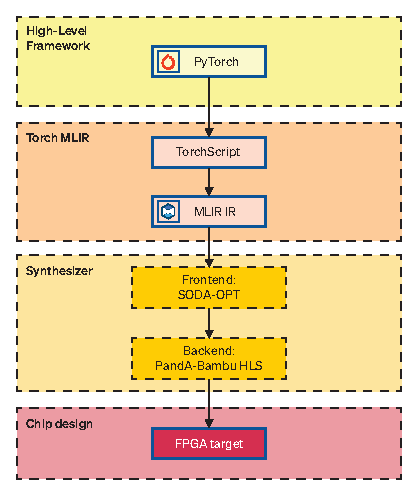
\includegraphics[height=0.6\textwidth]{Images/toolchain}
    \caption{FPGA Toolchain for Graph Neural Network Acceleration}
    \label{fig:toolchain}
\end{figure}

\section{PyTorch}
\label{sec:toolchain-pytorch}%

PyTorch~\cite{DBLP:journals/corr/abs-1912-01703} is an open-source deep learning framework widely used for building and training artificial neural networks for various machine learning tasks.

The first step of the toolchain is to design and implement the Graph Neural Network model in PyTorch.
Doing so involves defining the GNN model architecture and writing the necessary forward pass to compute node and graph-level representations.
Once having defined the model, the next step is training the GNN using standard PyTorch techniques, such as defining a loss function, setting up an optimizer, and performing backpropagation to optimize the model parameters.

\subsection{GNN models}
\label{subsec:gnn_models}%

Two main models have been used for this thesis: the Graph Isomorphism Network from OGB~\cite{NEURIPS2020_fb60d411, ogb_gnn_models}, written using PyTorch Geometric~\cite{DBLP:journals/corr/abs-1903-02428}, and the Graph Convolutional Network~\cite{DBLP:journals/corr/KipfW16, pygcn}, written using PyTorch~\cite{DBLP:journals/corr/abs-1912-01703}.

Most research and experiments have been conducted using the GCN model.
The GCN class, reported below, is characterized by two Graph Convolutional layers.

\begin{lstlisting}[language=Python,label={lst:gcn-class}]
import torch.nn as nn
import torch.nn.functional as F
from pygcn.layers import GraphConvolution

class GCN(nn.Module):
    def __init__(self, nfeat, nhid, nclass, dropout):
        super(GCN, self).__init__()

        self.gc1 = GraphConvolution(nfeat, nhid)
        self.gc1 = GraphConvolution(nhid, nclass)
        self.dropout = dropout

    def forward(self, x, adj):
        x = F.relu(self.gc1(x, adj))
        x = F.dropout(x, self.dropout, training=self.training)
        x = self.gc2(x, adj)
        return F.log_softmax(x, dim=1)
\end{lstlisting}

The forward function of each layer, reported below, is mainly characterized by two matrix multiplications.

\begin{lstlisting}[language=Python,label={lst:gcn-layer-forward}]

def forward(self, input, adj):
    support = torch.mm(input, self.weight)
    output = torch.spmm(adj, support)
    if self.bias is not None:
        return output + self.bias
    else:
        return output
\end{lstlisting}

\subsection{Datasets}
\label{subsec:gnn_datasets}%

OGB provides different datasets that can be used with their models.
The one used for this thesis is called \textit{ogbg-molhiv}, a molecular property prediction dataset.
In each graph representing a molecule, nodes correspond to atoms, and edges represent chemical bonds.
The input node features consist of nine dimensions, encompassing information like atomic number, formal charge, and whether the atom is part of a ring.
The binary classification task consists in achieving precise predictions of target molecular properties, for example, determining whether a molecule inhibits HIV replication or not.

The dataset used for the GCN model is the \textit{Cora} one.
This dataset contains 2708 scientific publications, categorized into one of the seven classes considered.
The citation network contains 5429 links.
Each publication in the dataset is represented by a binary-valued word vector, indicating the absence or presence of the corresponding word from a dictionary of 1433 unique words.
The task is a multiclass classification, in which, given a paper, the objective is to classify it into one of the seven classes correctly.

\section{Torch-MLIR}
\label{sec:toolchain-torch_mlir}%

Torch-MLIR~\cite{torch_mlir} offers compiler support for transitioning from the PyTorch ecosystem to the MLIR ecosystem.

The steps Torch-MLIR follows to go from PyTorch to MLIR are shown in Figure~\ref{fig:torch-mlir}.
In particular, the flow followed in this thesis has been highlighted with blue arrows.
There are two starting points of the flow: TorchScript and LazyTensorCode.
The one used for this research, which is also the most tested one, is TorchScript.
TorchScript~\cite{torchscript} offers a way to generate serializable and optimizable models directly from PyTorch code.

The TorchScript representation is then converted to MLIR using the built-in conversion of Torch-MLIR. The result MLIR can use different dialects, but the one used for this thesis is the Linalg dialect, which serves as input for the next phase of the toolchain.

\begin{figure}[t]
    \centering
    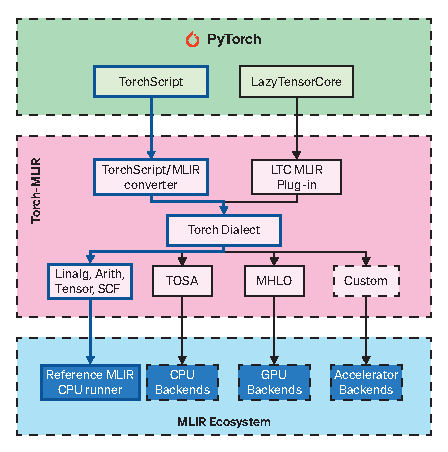
\includegraphics[height=0.5\textwidth]{Images/torch-mlir}
    \caption{Torch-MLIR flow}
    \label{fig:torch-mlir}
\end{figure}

\subsection{From PyTorch to TorchScript}
\label{subsec:pytorch-to-torchscript}%

Since Torch-MLIR implicitly uses the TorchScript representation to go from PyTorch to MLIR, the first part of the research consisted of a deep analysis of the Graph Neural Network models to make them compatible with TorchScript.

This task required more effort for the GIN model due to its use of PyTorch Geometric than the GCN model, which only uses pure PyTorch.
In particular, the required adaptations, that have been used for both models, have been made general aiming to make them versatile for various applications.
They are documented below, with a small example for each of them:

\begin{itemize}
    \item[-] The GNN layer class, if created as a subclass of the Message Passing class, must be marked as Jittable whenever it is used.
\begin{lstlisting}[language=Python,label={lst:jittable}]
self.convs.append(GINConv(emb_dim).jittable())
\end{lstlisting}
    \item[-] The propagate function, if used, need its parameters to be explicitly annotated using one of the two available options: through the definition of a dictionary or through a comment.
\begin{lstlisting}[language=Python,label={lst:propagate-annotation}]
propagate_type = {'x': Tensor, 'edge_attr': Tensor}
\end{lstlisting}
    \item[-] It can happen that TorchScript is not able to recognize the correct type of variables.
    In this case, it is necessary to use an assertion to explicitly declare that the variable is an instance of the correct type.
\begin{lstlisting}[language=Python,label={lst:isinstance-assertion}]
assert isinstance(edge_embedding, Tensor)
\end{lstlisting}
    \item[-] A common approach to speed up the training and inference steps is to use batched data.
    Unfortunately, TorchScript does not support forward functions that take as input a batch.
    For this reason, the forward function must receive Tensors as input, thus the batch must be split into its component.
\begin{lstlisting}[language=Python,label={lst:splitted-forward}]
def forward(self, x, edge_index, edge_attr):
\end{lstlisting}
    \item[-] The parameters of the forward function must be explicitly annotated with their type.
    If not declared, it is assumed to be of type Tensor.
\begin{lstlisting}[language=Python,label={lst:forward-annotation}]
def forward(self, x: Tensor, edge_index: Tensor,
            edge_attr: Tensor) -> Tensor:
\end{lstlisting}
    \item[-] TorchScript always expects an integer literal for the index, this is because indexing is only supported with integer literals.
    For this reason, cycles that do not use integer literals must be changed into enumeration.
\begin{lstlisting}[language=Python,label={lst:enumeration}]
for idx, layer in enumerate(self.convs):
\end{lstlisting}
\end{itemize}

\subsection{Torch-MLIR Compilation}
\label{subsec:torch-mlir-compilation}%

Once having designed, implemented, made compatible with TorchScript, and trained the GNN model in PyTorch, it is possible to use the \lstinline{torch_mlir.compile} API to obtain the MLIR representation of the model.
In particular, this API takes three parameters as input: the GNN model, an input example of the model and the desired output type.
The Graph Neural Network model must have been already trained, being ready for inference.
The second parameter, the input example of the model, is an arbitrary input similar to the one that would be given for inference purposes.
It is required because, by default, the implicit Jit function called by Torch-MLIR to script the model and obtain a script module, involves compiling the forward method and recursively compiling any methods, submodules, and functions called within the forward method. This results in a JIT IR which is converted to the torch dialect which is almost in a 1:1 correspondence.
The torch dialect is then lowered into one of the three available output dialects: linalg, tosa, mhlo.
The purpose of the last parameter is to choose which of these three dialects has to be used for the output MLIR.

An additional parameter that can be used is related to the tracing.
There are two ways in which it is possible to obtain a TorchScript representation: \lstinline{torch.jit.script} and \lstinline{torch.jit.tracing}.
The compile API of Torch-MLIR uses the first one by default.
Instead, if the option use tracing is set to True, JIT tracing is used.
The behavior of the two functions is slightly different.
Tracing only captures functions and modules that lack data dependencies and untracked external dependencies.
It records operations performed when the specified function is executed on the given tensors.
As a result, the resulting ScriptModule consistently executes the same traced graph for any input.
In conclusion, tracing can be a valid option in some cases, such as when there is no need to record any control-flow like if-statements or loops, but the scripting is preferred, and it is guaranteed to work in a more wide set of cases.
A call example of the compile Python API of Torch-MLIR is reported below.
\begin{lstlisting}[language=Python,label={lst:torch_mlir-compile}]
module = torch_mlir.compile(gnn_model, (x, features, adj),
                            output_type="linalg-on-tensors")
\end{lstlisting}

Once having obtained the compiled module, the expected behavior is to use one of the backends provided by torch-MLIR to make the inference.
This is not the flow followed in this thesis, because, as represented in the accelerator design flow, in Figure~\ref{fig:toolchain}, it is needed to export the Linalg representation for the next phase.
This can be done by simply saving the model to an MLIR file, as shown below.
\begin{lstlisting}[language=Python,label={lst:torch_mlir-export}]
with open("gnn_model.mlir", "w", encoding="utf-8") as outf:
    outf.write(str(module))
\end{lstlisting}

Only the GCN model implemented in PyTorch reached this phase of the toolchain.
During the research, much effort has been spent in trying to add support for the PyTorch Geometric framework to the toolchain.
Even if some innovation has been brought in this regard, there are still open points to work on.
For this reason, at the actual state, the proposed design flow only supports PyTorch as a high-level framework
It must be noted that no documentation existed and no previous works have ever used Torch-MLIR with GNN models.
All the examples and the work done by the Torch-MLIR community are related to Deep Neural Network models.

This thesis could represent the first work that explored the use of Torch-MLIR with GNN models.
Unfortunately, even if some innovation has been brought, such as the implementation of support of the constant of Tuple type, some more work is still required.
In particular, Torch-MLIR does not support the \lstinline{aten.scatter_add} operation, which, at the actual state, cannot be lowered to MLIR\@.
This operation is extensively used by PyTorch Geometric, leading to the incompatibility of the two elements.
The next step to add support for PyTorch Geometric to the proposed toolchain would be the implementation to Torch-MLIR of the lowering of the scatter add operation.

Another point discovered during this thesis is the fact that Torch-MLIR does not support the sparse tensor type. 
Each sparse tensor implemented in PyTorch, with the relative sparse operations, is lowered to MLIR to a dense tensor, losing all its representation's advantages.
A promising way to avoid this is Taco [??].
The MLIR team started creating what is called MLIR-PyTACO, an end-to-end use case for the sparse tensor compiler, which can be used to lower sparse Tensor to MLIR.
It is important to clarify that, as introduced in~\cite{Bik_2022}, sparse tensors are supported by MLIR, with a dedicated sparse tensor dialect that uses intuitive annotations for different sparse tensor representations, such as CSR and COO.
What is not supported yet is the lowering through Torch-MLIR\@.
However, MLIR-PyTACO is still premature and in testing phase, but interesting features could be brought by its advancement.

Even losing the sparse tensor representation, using the proper optimizations provided by the toolchain in combination with the higher computational performance of FPGAs, still make it possible to accelerate the GNN operations, as will be stated in the next Chapter.

\section{Synthesizer}
\label{sec:toolchain-synthesizer}%

The synthesizer represents the final step of the toolchain, which optimizes and synthesizes the MLIR representation, targeting FPGA\@.
This step includes SODA-OPT and PandA-Bambu, both introduced in Section~\ref{sec:soda}.
The following Subsections provide insight into what is happening internally to these two components.

\begin{figure}[t]
    \centering
    \subfloat[Compiler frontend\label{fig:soda-opt_flow}]{
        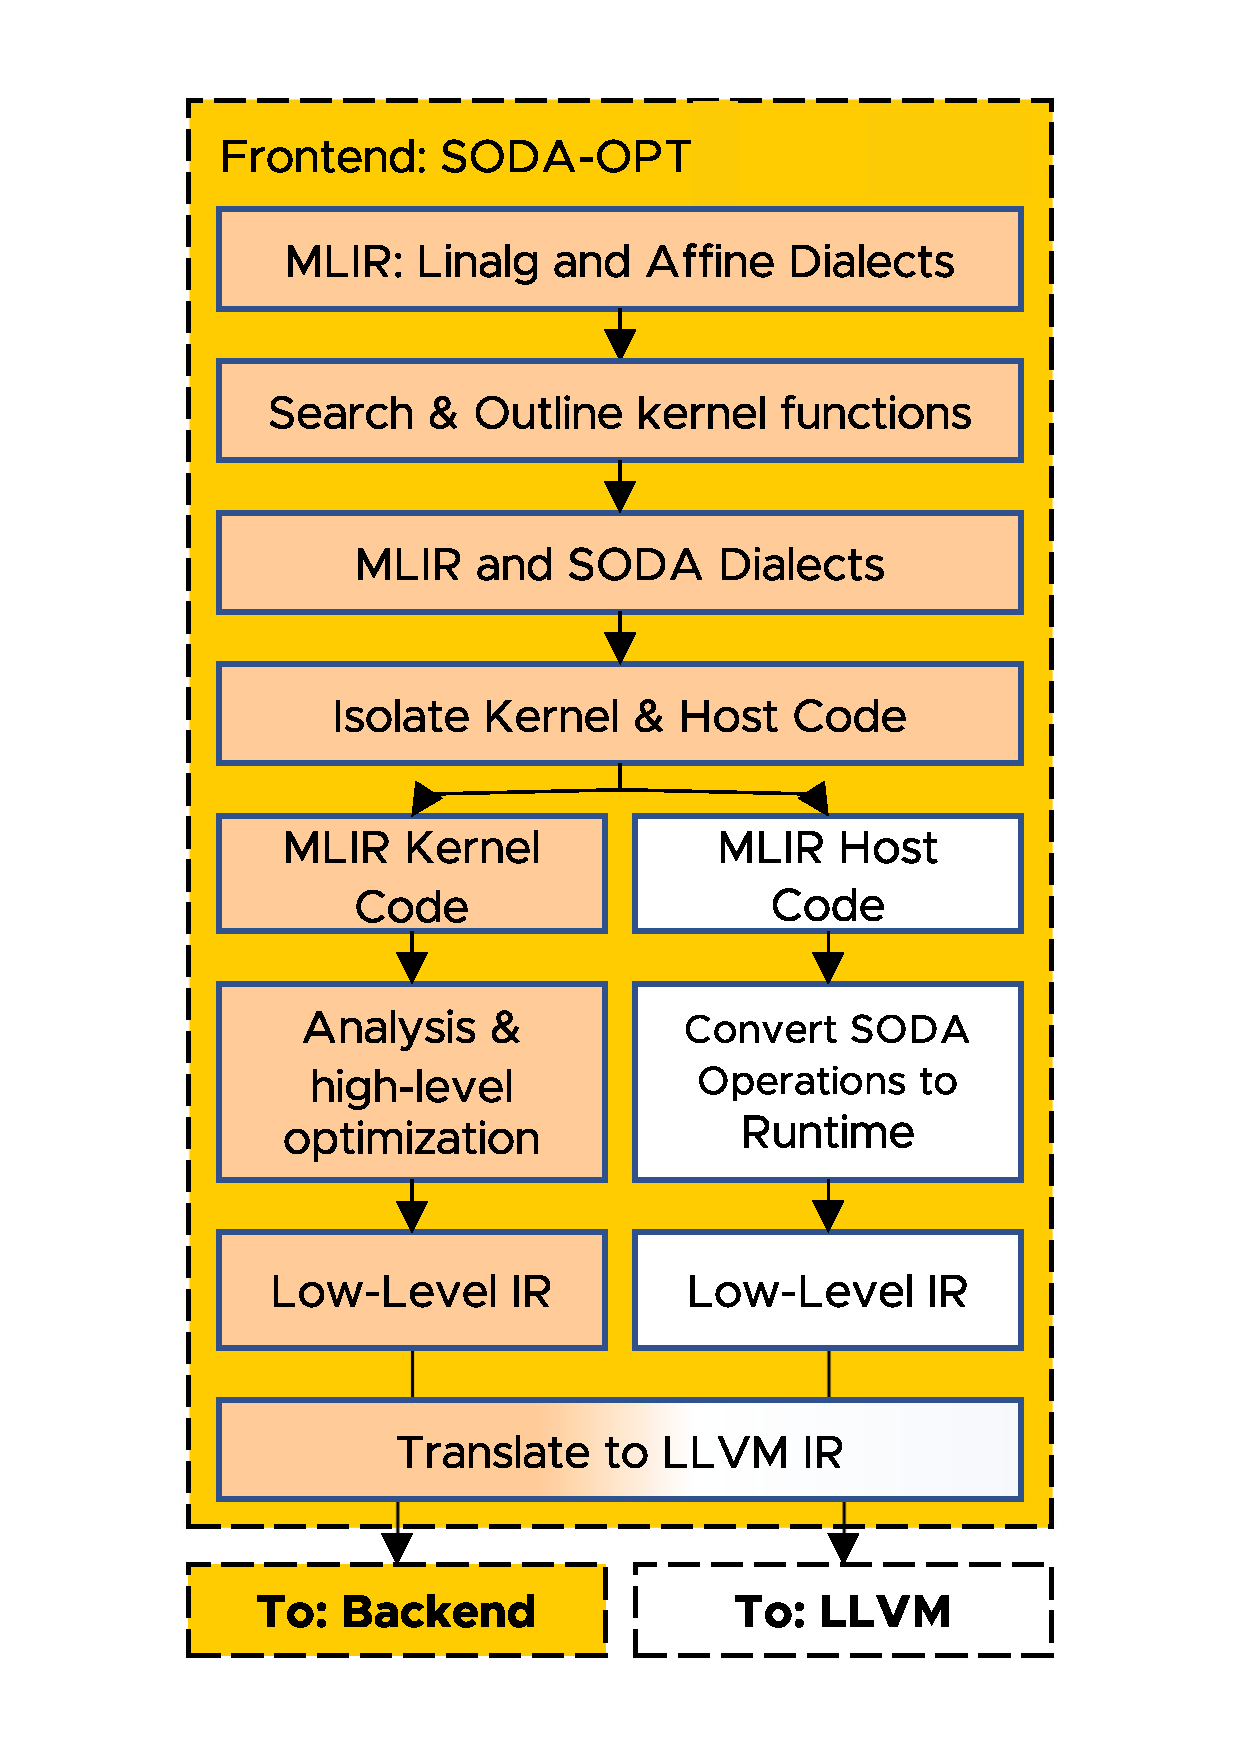
\includegraphics[height=0.5\textwidth]{Images/soda_opt_flow}
    }
    %\quad
    \hspace{0.03\textwidth}
    \subfloat[High-level synthesis backend\label{fig:bambu_flow}]{
        \captionsetup{width=.4\textwidth}
        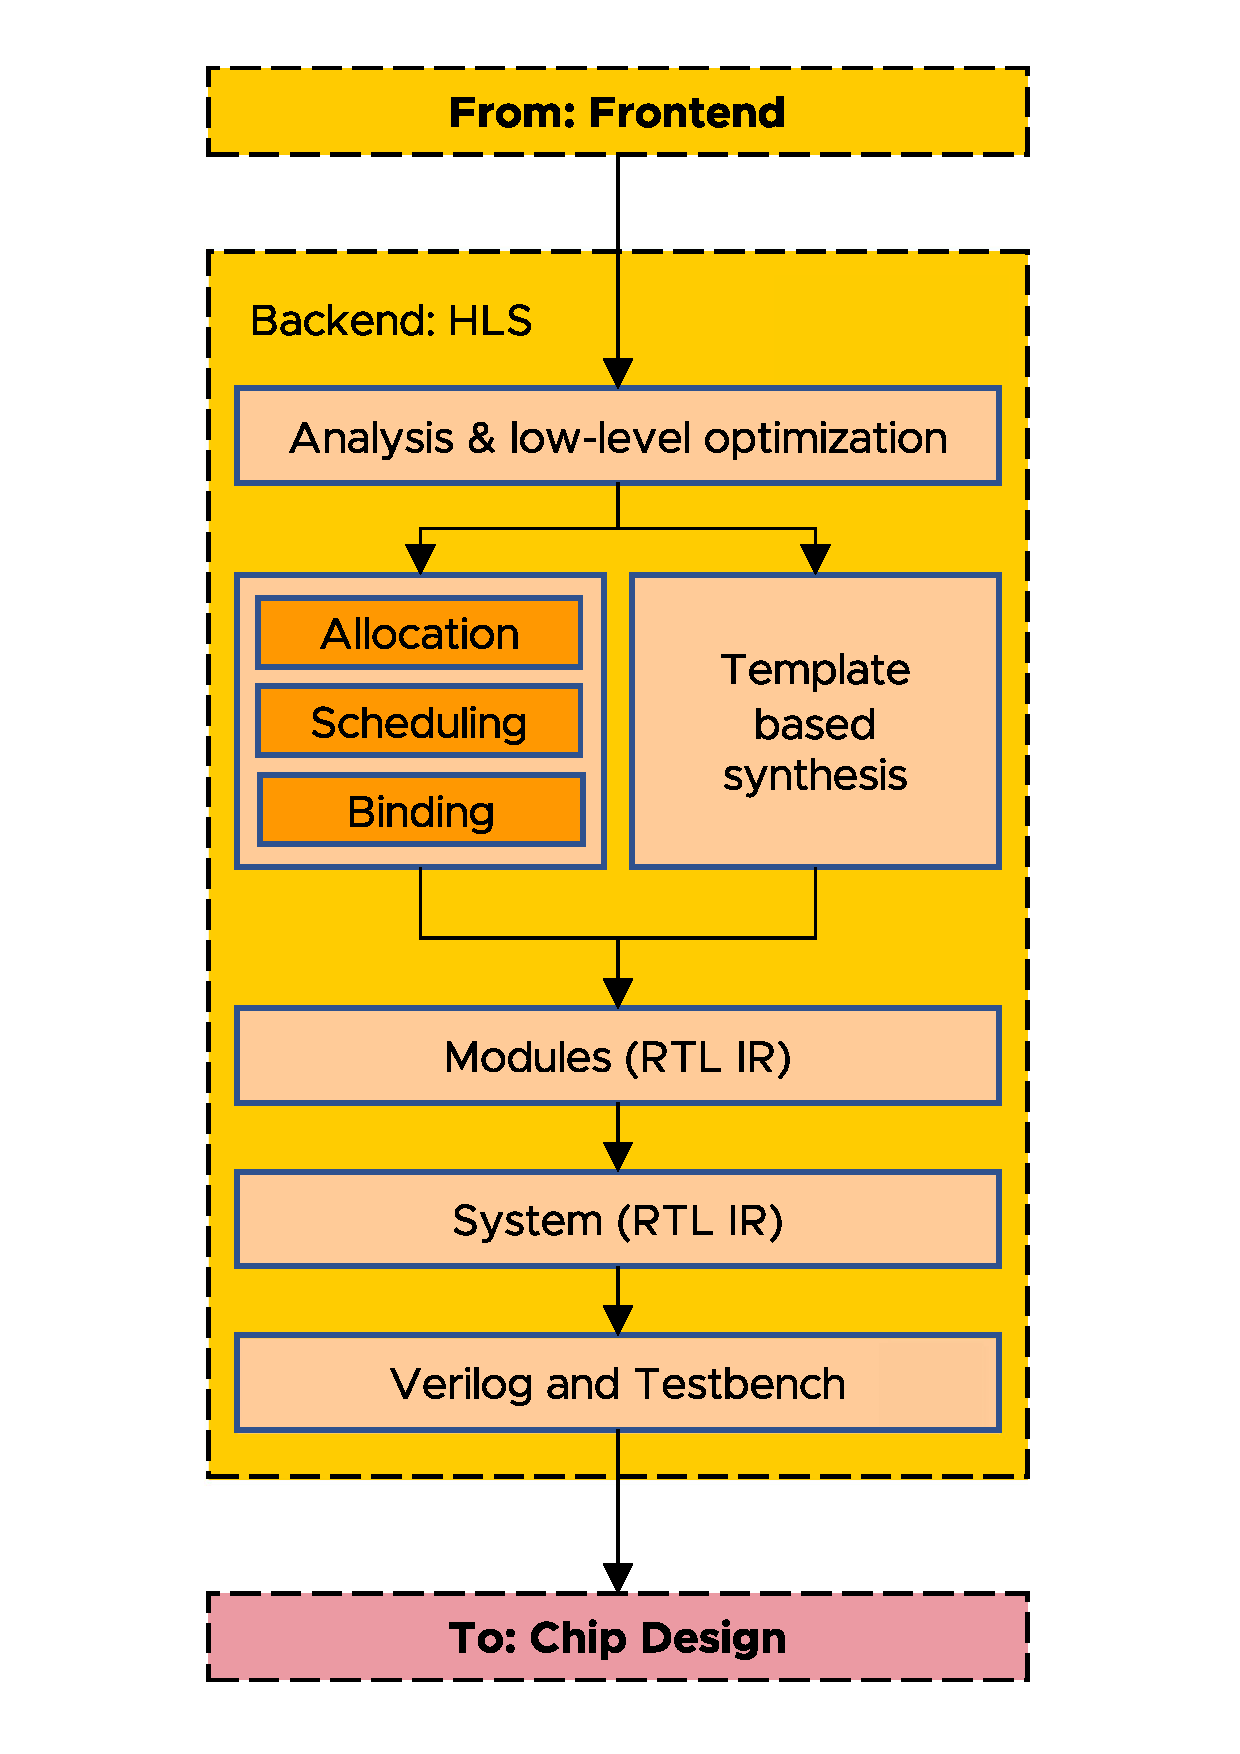
\includegraphics[height=0.5\textwidth]{Images/bambu_flow}
    }
    \caption{Synthesizer: SODA-OPT and PandA-Bambu overview~\cite{9786533}}
    \label{fig:synthesizer_flow}
\end{figure}

\subsection{SODA-OPT}
\label{subsec:toolchain-soda_opt}%

SODA-OPT, as shown in Figure~\ref{fig:soda-opt_flow}, receives as input the MLIR representation of the model.
This step is primarily responsible for applying optimizations that can be exploited in the next step.
In particular, a subset of MLIR passes can be used to do so.
The output of SODA-OPT is an LLVM representation that serves as input to PandA-Bambu HLS\@.

Despite the remarkable capabilities of SODA-OPT, it should be noted that it does not support the entire set of dialects utilized within the MLIR ecosystem, such as the ml\_program or the Tensor dialect.
Consequently, an additional step is required wherein the representation obtained from Torch-MLIR is lowered to remove unsupported dialects.
In particular, once having successfully exported the MLIR representation using the \lstinline{torch_mlir.compile} API, the mlir-opt passes shown below have been used to remove the unsupported dialects by lowering them to supported ones, such as the memref.

\begin{lstlisting}[language=bash,label={lst:mlir-opt-remove}]
mlir-opt --canonicalize -convert-tensor-to-linalg \
	     --empty-tensor-to-alloc-tensor --eliminate-empty-tensors \
	     -linalg-bufferize -arith-bufferize -tensor-bufferize -func-bufferize \
	     -finalizing-bufferize -buffer-deallocation --buffer-results-to-out-params \
	     --canonicalize -cse new_model.mlir
\end{lstlisting}

The next step consists in outlining the part of MLIR code to accelerate.
In general, the aim is to accelerate the whole function.
To do so, it is enough to modify the MLIR file by adding the \lstinline{soda.launch} and \lstinline{soda.terminator} flags at the beginning and end of the function, thus after the start of the forward and before the return statement.

SODA-OPT provides various passes that can be used to apply optimization to the outlined code.
In particular, it provides a subset of MLIR passes plus a set of passes tailored for soda optimizations.
The SODA-OPT passes are continuously evolving, trying to keep up with rapid advancement and innovation within the domain of MLIR\@.

An essential part of this research has been the analysis of the GNN model, the understanding of its bottlenecks, and the consequent identification of the optimization having the biggest impact on performance, without increasing too much the area of the accelerator.

The first part of this analysis has been conducted on PyTorch.
Profiling the inference function of the GCN model, the result showed that, in general, nearly 60\% of the time required to make a prediction was used for the matrix multiplication operation.
For this reason, an important part of this thesis is represented by research on how to accelerate matrix multiplication using SODA-OPT passes to then accelerate the GCN inference.

This analysis has been conducted using a subset of the Cora dataset, and the first pass used transforms the linalg to affine dialect, resulting in three nested affine loops shown below.

\begin{lstlisting}[label={lst:affine-mul}]
affine.for %arg3 = 0 to 15 {
affine.for %arg4 = 0 to 16 {
  affine.for %arg5 = 0 to 15 {
    %0 = affine.load %arg0[%arg3, %arg5] : memref<15x15xf32>
    %1 = affine.load %arg1[%arg5, %arg4] : memref<15x16xf32>
    %2 = affine.load %arg2[%arg3, %arg4] : memref<15x16xf32>
    %3 = arith.mulf %0, %1 : f32
    %4 = arith.addf %2, %3 : f32
    affine.store %4, %arg2[%arg3, %arg4] : memref<15x16xf32>
  }
}
}
\end{lstlisting}

The result of this research showed that the most impressive improvement in terms of performance is given by the loop unrolling technique.
This optimization perfectly allows to exploit the extreme parallelism available on FPGAs.
The right choice is not to continuously unroll until having no more loops in the code.
The solution is to pick the right trade-off between performance reduction and the area of the matrix multiplication accelerator.

%TODO: --mettere qualche nozione in più del flow di soda-opt, ad esempio come fa a prendere outline del kernel, la generazione dell'xml etc..-

\subsection{PandA-Bambu}
\label{subsec:toolchain-panda_bambu}%

PandA-Bambu represents the last phase of the synthesis.
As represented in Figure~\ref{fig:bambu_flow}, it receives the LLVM representation as input, and after having applied some optional low-level optimizations, it performs the typical steps of HLS introduced in Section~\ref{sec:hls}.

Then, after traversing through each stage of the proposed toolchain's process, the accelerator, i.e., the Bambu's output, represents the final output, tailored to target and maximize performance on cutting-edge FPGA architectures.

\section{Limitations}
\label{sec:toolchain-limitations}%

The most crucial advantage of the proposed toolchain is that it allows obtaining an accelerator without any knowledge of hardware design and implementation, starting directly from the PyTorch high-level framework.

During the research, much effort has been spent trying to add support for the PyTorch Geometric framework to the toolchain.
Unfortunately, even if some improvements have been reached, as the implementation of support of the constant of Tuple type, some obstacles are still present.
In particular, Torch-MLIR does not support \texttt{aten.scatter\_add} operation, which, at the actual state, cannot be lowered to MLIR\@.
This operation is extensively used by PyTorch Geometric, leading to the incompatibility of the two elements.

Another limitation is represented by the fact that Torch-MLIR does not support the sparse tensor type.
Each sparse tensor is lowered to a dense tensor, losing all this representation's advantages.
However, using the proper optimizations provided by the toolchain in combination with the higher computational performance of FPGAs, it is still possible to accelerate most of these operations, as discussed in the next Chapter.

Furthermore, despite the remarkable capabilities of SODA-OPT, it should be noted that it does not support the entire set of dialects utilized within the MLIR ecosystem, such as the Tensor dialect.
Consequently, this limitation requires an additional step wherein the representation is lowered to remove unsupported dialects.
In addition to the dialect limitation, SODA-OPT only supports a subset of MLIR passes.
The reason behind this restriction lies in the rapid advancement and innovation within the domain of MLIR\@.

These limitations are not trivial but do not prevent the achievement of the acceleration objective and do not compromise the proposed solution's capability.



% ##########################################################################
% CHAPTER SIX - EXPERIMENTAL RESULTS
% ##########################################################################


    \chapter{Experimental Procedures and Results}
    \label{ch:chapter_six}%
    This Chapter presents all the experiments performed and the achieved results.
Firstly, some theoretical aspects of each experimental phase are introduced, then all the experiments are clearly illustrated to make them reproducible and the obtained results are explained.

All the CPU experiments have been conducted using an Intel Core i9, with 8 cores and a frequency of 2,3 GHz.
On the other hand, the synthesis experiments utilized an AMD Virtex UltraScale+ (Alveo U280) FPGA\@.

\section{Model analysis and profiling}
\label{sec:model-analysis}%

\begin{table}[b]
\centering
    \begin{tabular}{|p{6em} c c c c|}
    \hline
%    \rowcolor{black!40}
    \textbf{Name} & \textbf{Self CPU \%} & \textbf{Self CPU} & \textbf{CPU total \%} & \textbf{CPU total} \T\B \\
    \hline \hline
    \textbf{aten::mm} & 50,25\% & 1,012$ms$ & 89,72\% & 1,807$ms$ \T\B\\
    \hline
    \textbf{aten::addmm} & 36,30\% & 731,0$\mu s$ & 37,04\% & 746,0$\mu s$ \T\B\\
    \hline
    \textbf{aten::add} & 4,67\% & 94,0$\mu s$ & 4,67\% & 94,0$\mu s$ \T\B\\
    \hline
    %\textbf{aten::\_log\_softmax} & 2,98\% & 60,0us & 2,98\% & 60,0us \T\B\\
    %\hline
    \end{tabular}
    \\[10pt]
    \caption{Excerpt of GCN model inference profiling result}
    \label{tab:gcn_profiling}
\end{table}

As already anticipated in Section~\ref{sec:toolchain-pytorch}, the GCN model, whose class is shown in Listing~\ref{lst:gcn-class}, is implemented in PyTorch, and it is characterized by two convolutional layers, a ReLU and a dropout functions.
The forward function of each layer, shown in Listing~\ref{lst:gcn-layer-forward}, is characterized by two matrix multiplications, and one of the two is a sparse multiplication.

The first step to understanding how to accelerate the PyTorch GCN model used was to analyze and profile it.
Table~\ref{tab:gcn_profiling} shows the results of one result of the profiling done using the PyTorch profiler.

The distinction between \textit{self CPU time} and \textit{total CPU time} lies in the fact that self CPU time does not contain the time spent in child operator calls, whereas total CPU time contains it, considering that operators can invoke other operators.
It is clear that the bottleneck and the most time-consuming operation is the matrix multiplication.
In particular, more than 50\% of the self CPU time is used by matrix multiplication, while, considering the child operator calls, this percentage represents nearly the 90\%.
This result clearly justifies the part of this research dedicated to matrix multiplication acceleration.

\begin{lstlisting}[language=Python,label={lst:gcn-class}, numbers=left, xleftmargin=2em, caption=Class of GCN model]
import torch.nn as nn
import torch.nn.functional as F
from pygcn.layers import GraphConvolution

class GCN(nn.Module):
    def __init__(self, nfeat, nhid, nclass, dropout):
        super(GCN, self).__init__()

        self.gc1 = GraphConvolution(nfeat, nhid)
        self.gc1 = GraphConvolution(nhid, nclass)
        self.dropout = dropout

    def forward(self, x, adj):
        x = F.relu(self.gc1(x, adj))
        x = F.dropout(x, self.dropout,
                      training=self.training)
        x = self.gc2(x, adj)
        return F.log_softmax(x, dim=1)
\end{lstlisting}


\begin{lstlisting}[language=Python,label={lst:gcn-layer-forward}, numbers=left, xleftmargin=2em, caption=Forward function of GCN layer]
    def forward(self, input, adj):
        support = torch.mm(input, self.weight)
        output = torch.spmm(adj, support)
        if self.bias is not None:
            return output + self.bias
        else:
            return output
\end{lstlisting}

\section{Matrix multiplication acceleration}
\label{sec:matmul-acceleration}%

Matrix multiplication is a well-known algorithm.
It consists of multiplying two compatible matrices to obtain the result matrix.
A lot of work has been done to try to improve its performance on different architectures~\cite{DBLP:journals/corr/abs-2003-00532, opt_cuda_matmul}.

The naive implementation of the row-by-column multiplication, whose pseudocode is shown below, is characterized by three nested loops.
The multiplication is possible only in the case the number of column of the first matrix is equal to the number of row of the second one.

\begin{algorithm}[H]
    \label{alg:matmul_pseudo}
    \caption{Naive matrix multiplication algorithm}
    \label{alg:var}
    \label{protocol1}
    \begin{algorithmic}[1]
    \STATE \textbf{Data:} $A[R][P], B[M][N]$
    \STATE \textbf{Result:} $C[R][N]$
    \IF{$P == M$}
    \FOR{$m=0; m<R, m++$}
    \FOR{$r=0; r<N, r++$}
    \STATE $C[m][r] = 0$
    \FOR{$k=0; k<M, k++$}
    \STATE $C[m][r] += A[m][k] * B[k][r]$
    \ENDFOR
    \ENDFOR
    \ENDFOR
    \ENDIF
    \end{algorithmic}
\end{algorithm}

\begin{figure}[t]
    \centering
    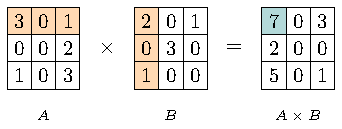
\includegraphics[height=0.24\textwidth]{Images/row-by-col-mult-example}
    \caption{Row-by-column matrix multiplication example}
    \label{fig:row-by-col-mul-example}
\end{figure}

Figure~\ref{fig:row-by-col-mul-example} highlight how an element of the output matrix is computed, using a row of the first matrix and a column of the second one.
The number of operations needed to compute a new matrix is an important parameter to try to accelerate such operation.
A calculus of this number preceded each experiments, to compute an approximation of the number of cycles needed by the accelerator.
In a general matrix multiplication, shown in Equation~\ref{eq:matmul}, each element of the new matrix can be computed accordingly to Equation~\ref{eq:matmul-element}.

\begin{equation}
        \label{eq:matmul}
    \begin{bmatrix}
     a_{11} & a_{12} & \cdots & a_{1n}\\
     a_{21} & a_{22} & \cdots & a_{2n}\\
     \vdots & \vdots & \ddots & \vdots\\
     a_{m1} & a_{m2} & \cdots & a_{mn}
 \end{bmatrix}
 \times
 \begin{bmatrix}
     b_{11} & b_{12} & \cdots & b_{1p}\\
     b_{21} & b_{22} & \cdots & b_{2p}\\
     \vdots & \vdots & \ddots & \vdots\\
     b_{n1} & b_{n2} & \cdots & b_{np}
 \end{bmatrix}
  =
 \begin{bmatrix}
     c_{11} & c_{12} & \cdots & c_{1p}\\
     c_{21} & c_{22} & \cdots & c_{2p}\\
     \vdots & \vdots & \ddots & \vdots\\
     c_{m1} & c_{m2} & \cdots & c_{mp}
 \end{bmatrix}
\end{equation}

\begin{equation}
    \label{eq:matmul-element}
    c_{ij}= a_{i1} b_{1j} + a_{i2} b_{2j} +\cdots+ a_{in} b_{nj} = \sum_{k=1}^n a_{ik}b_{kj}
\end{equation}

Then, the number of cycles needed can be calculated using Equation~\ref{eq:number-cycles}.
The notation used refers to Equation~\ref{eq:matmul}, but it can be referred to Algorithm~\ref{alg:var} by considering $n = M \land m=R \land p=N$
The first part of the Equation computes the total number of iterations, while the second half computes the number of cycles needed to perform multiplications and additions, and to load and store data.
The number of cycles needed to load and store data are computed by adding one cycle for each $ch$ operands read, and one cycle for each $ch$ operand written, with $ch$ equal to the number of memory channels.
From Listing~\ref{lst:affine-mul}, it can be seen that there are three load and one store, for a total of four memory operations.

\begin{equation}
    \label{eq:number-cycles}
    cycles = \left(  n \cdot m \cdot p \right) \cdot \left(  cycles_{mul} + cycles_{add} + \frac{4}{ch} \right)
\end{equation}

Let us consider two matrices, the first of size $15\times15$ and the second of size $15\times16$.
The FPGA model used for the experimental phase uses three cycles for addition and two cycles for multiplication.
By applying the Equation~\ref{eq:number-cycles}, the expected number of cycles for computing such matrix multiplication, using two memory channels is 25,200.

\subsection{PyTorch matrix multiplication benchmark}
\label{subsec:pytorch-matmul-bench}%

PyTorch provides different matrix representations and different matrix multiplication functions.
The one considered in this Subsection are \textit{torch.mm} and \textit{torch.spmm}.
The former function multiplies two dense matrices, but it also supports COO representation.
The latter, instead, is typically used for sparse matrix multiplications, in which one of the two matrices, or both, are saved using sparse representations.

Figure~\ref{fig:torch-mm_benchmark} represents a benchmark for the dense matrix multiplication between a first matrix of size $15 \times 15$ and a second matrix of size $15 \times 16$, both composed by float32 elements.
In particular, the plot shows five measurements computed as the average of five different executions' number.
Additionally, this average has been computed five times, and the red bar shows the range between the minimum and the maximum execution time of these repetitions.

As expected, given the high amount of executions, the five average execution times are similar between them, and the red range bar decreases as the number of executions increases.
In conclusion, the time needed by a dense matrix multiplication between two matrices of the given size can be considered equal to 1.608$\mu s$.
The Python timing of the accelerated functions for each experiment has been computed using an average of ten millions executions.

Since the GCN model uses both dense and sparse matrix multiplication functions, Table~\ref{tab:torch-matmul-comparison} shows the times needed by both functions according to different representations of the two input matrices A and B\@.
All the times have been computed as the average of ten millions executions, the two matrices are both of size $20 \times 20$ and randomly generated; they are both composed by float32 elements and COO matrices have a sparsity of 90\%.

\begin{table}[t]
\centering
    \begin{tabular}{|p{6em} c c c |}
    \hline
    \textbf{Function} & \textbf{Dense$\times$Dense} & \textbf{COO$\times$Dense} & \textbf{COO$\times$COO} \T\B \\
    \hline \hline
    \textbf{torch.mm} & 1.840$\mu s$  & 3.299$\mu s$ & 16.855$\mu s$ \T\B\\
    \hline
    \textbf{torch.spmm} & 1.875$\mu s$  & 3.234$\mu s$ & 15.215$\mu s$ \T\B\\
    \hline
    \end{tabular}
    \\[10pt]
    \caption{Comparison between dense and sparse PyTorch matmul functions}
    \label{tab:torch-matmul-comparison}
\end{table}

\begin{figure}[t]
    \centering
    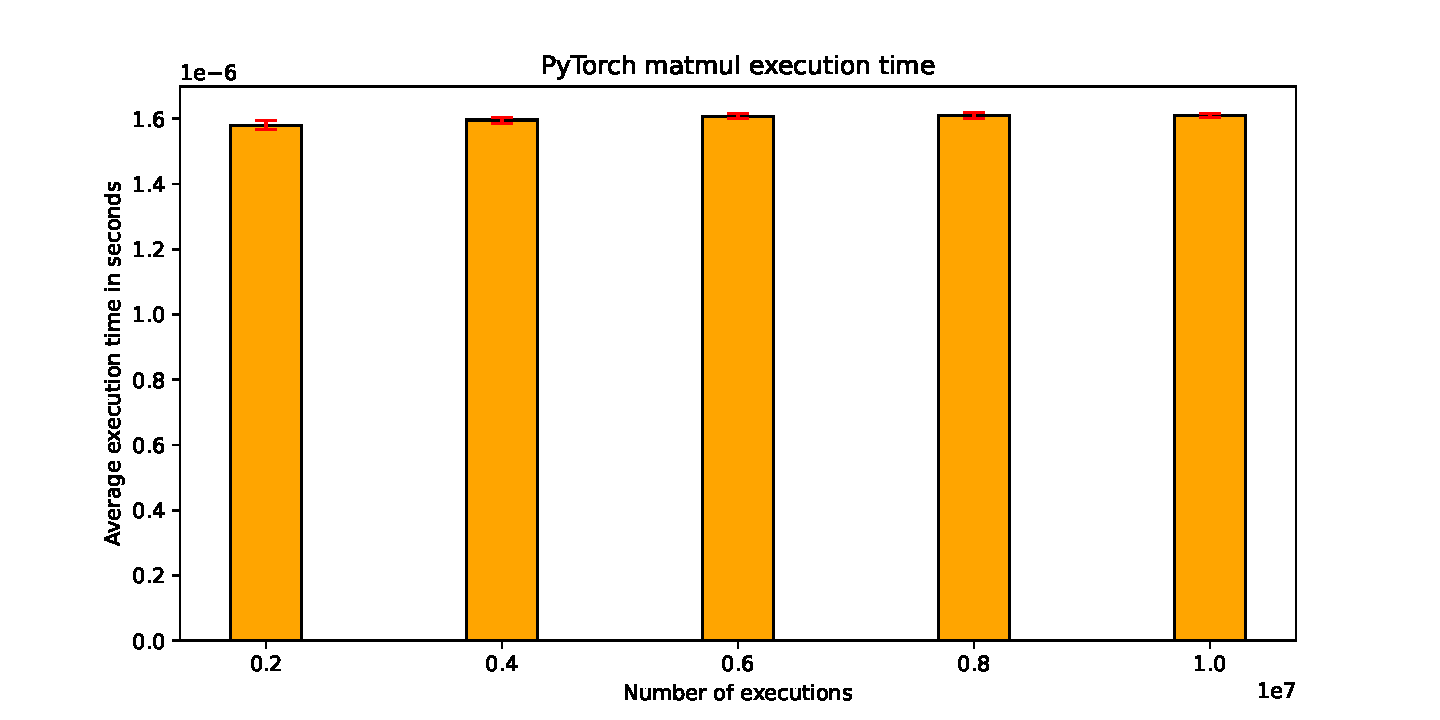
\includegraphics[height=0.4\textwidth]{Images/torch-mm_benchmark}
    \caption{Benchmark of \textit{torch.mm} PyTorch function}
    \label{fig:torch-mm_benchmark}
\end{figure}

It is clear that sparse matrix multiplication, both with dense and sparse matrix representations, does not increase performance on CPU architecture.
The disadvantage of using sparse matrix multiplication on CPU becomes more and more evident as the size of the input matrices increases.

\subsection{Optimization comparison}
\label{subsec:optimization-comparison}%

Before applying any SODA-OPT or PandA-Bambu optimization, it is necessary to understand the difference between PyTorch matrix multiplication operation and the baseline accelerator.
Table~\ref{tab:pytorch-accelerator-comparison} and Figure~\ref{fig:pytorch-accelerator-comparison} show the result of this analysis.
The PyTorch times have been recorded by averaging five measurements each of ten millions executions.
The baseline accelerator is much faster than PyTorch when matrices are relatively small.
The difference of performance decreases as the size of the input matrices increase until reaching a point in which the accelerator becomes slower than PyTorch solution.

\begin{table}[t]
\centering
    \begin{tabular}{|p{9em} c c c c  |}
    \hline
    \textbf{Input sizes} & \textbf{Torch.mm (s)} & \textbf{Runtime (s)} & \textbf{Cycles} & \textbf{SpeedUp} \T\B \\
    \hline \hline
    \textbf{15$\times$15, 15$\times$16} & 1.608E-06  & 96.492E-09 & 25,697 & 16.664 \T\B\\
    \hline
    \textbf{30$\times$30, 30$\times$16} & 1.733E-06  & 351.182E-09 & 101,792 & 4.934 \T\B\\
    \hline
    \textbf{60$\times$60, 60$\times$16} & 2.480E-06  & 1.466E-06 & 405,182 & 1.691 \T\B\\
    \hline
    \textbf{90$\times$90, 90$\times$16} & 4.554E-06  & 3.150E-06 & 910,172 & 1.445 \T\B\\
    \hline
    \textbf{120$\times$120, 120$\times$16} & 4.792E-06  & 00.000E-06 & 00,000 & 16.664 \T\B\\
    \hline
    \textbf{150$\times$150, 150$\times$16} & 5.161E-06  & 9.074E-06 & 2,524,952 & 0.568 \T\B\\
    \hline
    \end{tabular}
    \\[10pt]
    \caption{Comparison between dense and sparse PyTorch matmul functions}
    \label{tab:pytorch-accelerator-comparison}
\end{table}

\begin{figure}[t]
    \centering
    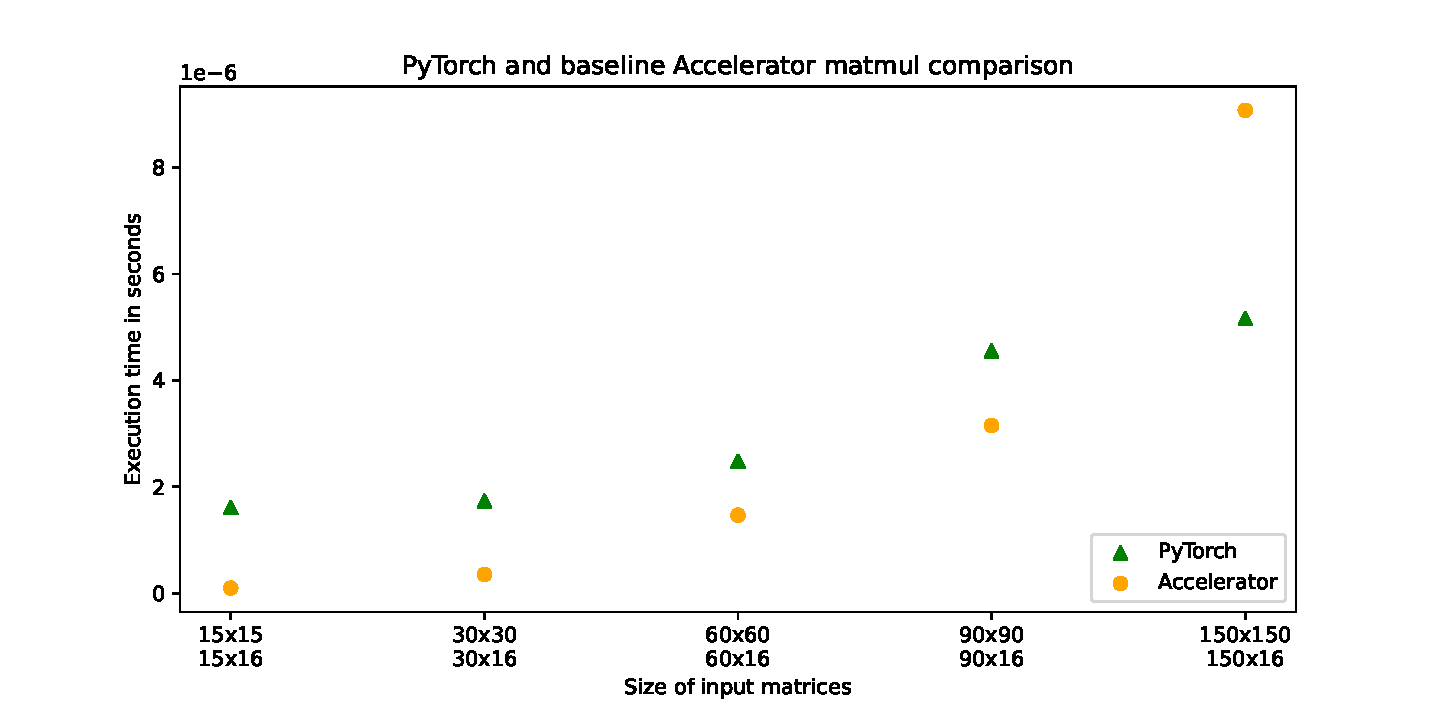
\includegraphics[height=0.4\textwidth]{Images/matmul_comparison}
    \caption{Performance comparison between PyTorch matmul function and accelerator}
    \label{fig:pytorch-accelerator-comparison}
\end{figure}

\begin{lstlisting}[label={lst:affine-mul-unroll3}, caption=Unrolled matrix multiplication in affine dialect with unrolling factor 3]
affine.for %arg3 = 0 to 15 {
  affine.for %arg4 = 0 to 16 {
    affine.for %arg5 = 0 to 15 step 3 {
      %0 = affine.load %arg0[%arg3, %arg5] : memref<15x15xf32>
      %1 = affine.load %arg1[%arg5, %arg4] : memref<15x16xf32>
      %2 = affine.load %arg2[%arg3, %arg4] : memref<15x16xf32>
      %3 = arith.mulf %0, %1 : f32
      %4 = arith.addf %2, %3 : f32
      affine.store %4, %arg2[%arg3, %arg4] : memref<15x16xf32>
      %5 = affine.apply affine_map<(d0) -> (d0 + 1)>(%arg5)
      %6 = affine.load %arg0[%arg3, %5] : memref<15x15xf32>
      %7 = affine.load %arg1[%5, %arg4] : memref<15x16xf32>
      %8 = affine.load %arg2[%arg3, %arg4] : memref<15x16xf32>
      %9 = arith.mulf %6, %7 : f32
      %10 = arith.addf %8, %9 : f32
      affine.store %10, %arg2[%arg3, %arg4] : memref<15x16xf32>
      %11 = affine.apply affine_map<(d0) -> (d0 + 2)>(%arg5)
      %12 = affine.load %arg0[%arg3, %11] : memref<15x15xf32>
      %13 = affine.load %arg1[%11, %arg4] : memref<15x16xf32>
      %14 = affine.load %arg2[%arg3, %arg4] : memref<15x16xf32>
      %15 = arith.mulf %12, %13 : f32
      %16 = arith.addf %14, %15 : f32
      affine.store %16, %arg2[%arg3, %arg4] : memref<15x16xf32>
    }
  }
}
\end{lstlisting}

This behaviour can be attributed to the fact that PyTorch times have been recorded using all the eight available threads on the machine.
So, the \lstinline{torch.mm} function exploits more parallelism with respect to the accelerator.
For this reason, the optimizations discussed in Section~\ref{subsec:toolchain-soda_opt} and in Section~\ref{subsec:toolchain-panda_bambu} and evaluated in the following makes the accelerator able to exploit more parallelism.

To verify the effectiveness of the proposed optimizations, different comparative analysis have been performed.
SODA-OPT offers the possibility to make different types of unrolling, among which the full unroll which completely unroll the innermost loop, and the partial unroll up to an arbitrary factor.
Listing~\ref{lst:affine-mul-unroll3} shows the effect of a partial unrolling, with unrolling factor equal to 3, to the matrix multiplication introduced in Listing~\ref{lst:affine-mul}.

PandA-Bambu introduces several optimization options, one of which involves expanding the number of memory channels in use.
By default, the system employs two channels and utilizes \lstinline{ALL_BRAM} as the memory allocation policy, directing all objects to be stored in BRAMs.
However, there's an alternative approach explored in this thesis, which entails employing a greater number of memory channels while utilizing external memory, approach that appears to be in line with the coalescent accesses performed on CUDA.
To achieve this, the \lstinline{NO_BRAM} memory allocation policy must be selected, leading to all objects being stored in external memory.

This choice offers both advantages and disadvantages, resulting in a trade-off.
Loop unrolling enhances parallelization, thereby reducing computational time.
However, especially when utilizing more than two memory channels, it increases the number of parallel processing elements, leading to a larger area footprint.
Additionally, external memory allows for up to 32 memory channels, enabling the simultaneous loading of 32 variables.
Nonetheless, accessing data from external memory requires more load cycles compared to accessing internal memory.

The conducted analyses aim to highlight the differences among these various configurations, identifying the optimal balance between reducing cycles and containing area utilization.

\begin{figure}[t]
    \centering
    \subfloat[Input matrices $15\times15$, $15\times16$\label{fig:matmul-optimization-comparison15}]{
        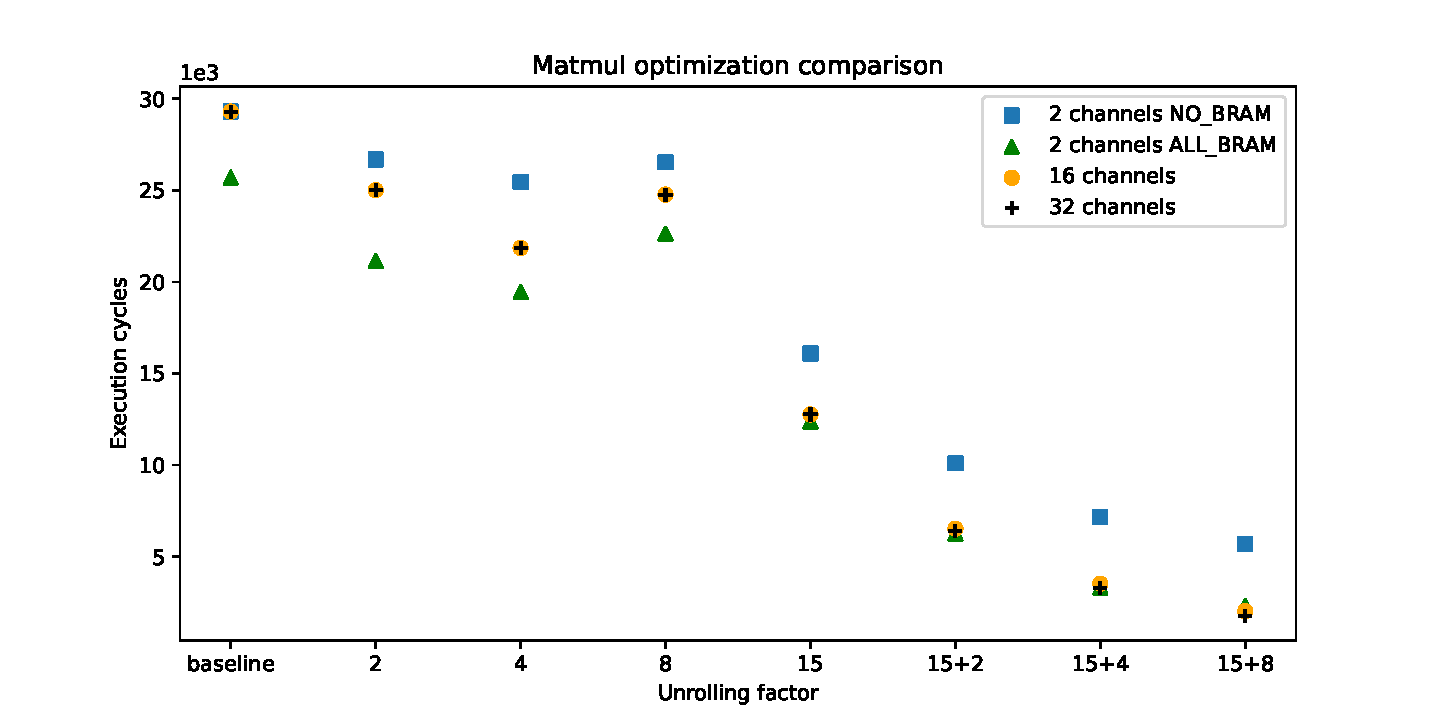
\includegraphics[height=0.4\textwidth]{Images/matmul_comparison15}
    }
    %\quad
    \hspace{0.15\textwidth}
    \subfloat[Input matrices $30\times30$, $30\times16$\label{fig:matmul-optimization-comparison30}]{
        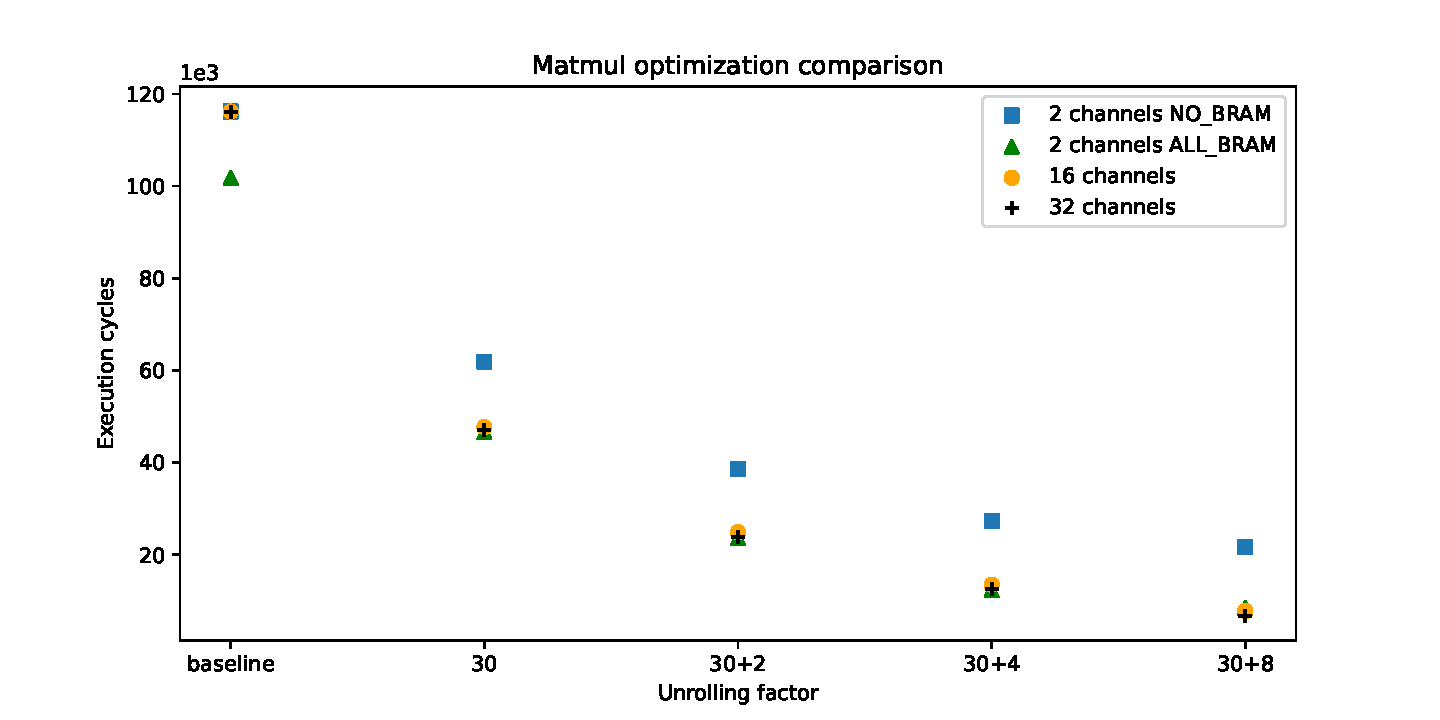
\includegraphics[height=0.4\textwidth]{Images/matmul_comparison30}
    }
    \caption{Matrix multiplication optimization comparison}
    \label{fig:matmul-optimization-comparison}
\end{figure}

Figure~\ref{fig:matmul-optimization-comparison} show two matrix multiplication analyzes performed using different sizes of the input matrices.
Figure~\ref{fig:matmul-optimization-comparison15} show results of a multiplication between two matrices of size $15\times15$ and $15\times16$, while Figure~\ref{fig:matmul-optimization-comparison30} shows results of a multiplication between two matrices of size $30\times30$ and $30\times15$.
In both figures, on the abscissa there is the unrolling factor used and on the ordinate the resulting number of cycles.
The baseline computation does not use unrolling, instead when there are two factors it means that the first one can be considered as a full unroll of the innermost cycle, while the second one is the unrolling factor applied to the original second innermost cycle.

In both cases, when the parallelization is not high, thus the unrolling factor is small, using two channels is the best option since a minor number of cycles is required to perform the computation.
Using 16 channels seems to be similar to use 32 channels, but when parallelization is high the former option uses fewer cycles.

The most important result is given by the unrolling factor in which the number of cycles needed by the accelerator using 32 memory channels is fewer than the number of cycles needed by the accelerator using 2 memory channels.
In the first case, in Figure~\ref{fig:matmul-optimization-comparison15}, this objective is achieved with two unrolling factors of 15 and 8, while in the second case is achieved with unrolling factors of 30 and 8.

These two results, since the unrolling factors are not equals, could appear unrelated.
Using 15 and 8 as unrolling factors means having $15 \cdot 8 = 120$ parallel loop iterations.
Instead, using 30 and 8 as unrolling factors means having $30 \cdot 8 = 240$ parallel loop iterations.

The total amount of possible parallel loop iterations in a matrix multiplication between two matrices of sizes $15\times15$ and $15\times16$ is equal to $15 \cdot 16 \cdot 15 = 3,600$.
Meanwhile, the total amount of possible parallel loop iterations in a matrix multiplication between two matrices of sizes $30\times30$ and $30\times16$ is $30 \cdot 16 \cdot 30 = 14,400$.

Even if the two number of parallel loop iterations representing the changing point of the trade-off, 120 and 240, are different, they are related by the following Equation:
\begin{equation}
    \label{eq:factor-relation}
        2 \cdot \sqrt {M \cdot N \cdot R} = i \cdot j \cdot k
\end{equation}

where $M$, $N$ and $R$ are the sizes of the three nested loops, as defined in Algorithm~\ref{alg:var}, and $i$, $j$ and $k$ are their respective loop unrolling factors, following the rule $j \neq 1 \iff i=M \land k \neq 1 \iff j=N$.

Equation~\ref{eq:factor-relation} should not be taken as an infallible rule, it is the outcome of this experimental phase and should be used as a discriminant to decide when to use thirty-two memory channels instead of two.
In conclusion, the generalized rule, outcome of this comparative analysis is that using thirty-two channels is preferred and convenient when the number of parallel loop iterations is greater than the one computed using Equation~\ref{eq:factor-relation}.

\subsection{GCN accelerator evaluation}
\label{subsec:gcn_accelerator_evaluation}%

\begin{table}[t]
\centering
    \begin{tabular}{|p{4em} c c c c c|}
    \hline
    \textbf{Name} & \textbf{Nodes} & \textbf{Words} & \textbf{Links} & \textbf{Task} & \textbf{Classes} \T\B \\
    \hline \hline
    \textbf{Cora} & 2708  & 1433 & 5429 & Multiclass classification & 7 \T\B\\
    \hline
    \textbf{Cora15} & 15  & 15 & 3 & Multiclass classification & 7 \T\B\\
    \hline
    \textbf{Cora30} & 30  & 30 & 4 & Multiclass classification & 7 \T\B\\
    \hline
    \textbf{Cora60} & 60  & 60 & 8 & Multiclass classification & 7 \T\B\\
    \hline
    \textbf{Cora90} & 90  & 90 & 18 & Multiclass classification & 7 \T\B\\
    \hline
    \textbf{Cora120} & 120  & 120 & 22 & Multiclass classification & 7 \T\B\\
    \hline
    \textbf{Cora150} & 150  & 150 & 37 & Multiclass classification & 7 \T\B\\
    \hline
    \end{tabular}
    \\[10pt]
    \caption{Cora sub-dataset used for GCN infernce}
    \label{tab:dataset-definition}
\end{table}

In this Subsection, the ultimate evaluation of the optimizations examined and suggested in Subsection~\ref{subsec:optimization-comparison} is presented, aimed at understanding their influence on GCN inference time.

As previously mentioned in the previous Subsection, Table~\ref{tab:pytorch-accelerator-comparison} shows the cycle counts required by the accelerator for each experiment.
These counts align perfectly with the anticipated expectations outlined in Equation~\ref{eq:number-cycles}.
Specifically, dividing the cycle count of the first experiment of the table and the final one by the total count of loop iterations effectively confirms a consistent result of approximately 7 in both instances, confirming that the number of cycles per each loop iteration stayed constant.

\begin{table}[t]
\centering
    \resizebox{\textwidth}{!}{
    \begin{tabular}{|p{4em} c c c c c c|}
    \hline
    \thead{Dataset} & \thead{PyTorch (s)} & \thead{Optimizations} & \thead{Runtime (s)} & \thead{Cycles} & \thead{Area} & \thead{SpeedUp} \T\B \\
    \hline \hline
    \makecell{Cora15} & 59.25E-06 & \makecell{32 channels \\ Unrolling} & 0E-09 & 0 & 0 & 0 \T\B\\
    \hline
    \makecell{Cora30} & 66.42E-06 & \makecell{32 channels \\ Unrolling} & 0E-09 & 0 & 0 & 0 \T\B\\
    \hline
    \makecell{Cora60} & 69.75E-06 & \makecell{32 channels \\ Unrolling} & 0E-09 & 0 & 0 & 0 \T\B\\
    \hline
    \makecell{Cora90} & 88.88E-06 & \makecell{32 channels \\ Unrolling} & 0E-09 & 0 & 0 & 0 \T\B\\
    \hline
    \makecell{Cora120} & 98.32E-06 & \makecell{32 channels \\ Unrolling} & 0E-09 & 0 & 0 & 0 \T\B\\
    \hline
    \makecell{Cora150} & 115.03E-06 & \makecell{32 channels \\ Unrolling} & 0E-09 & 0 & 0 & 0 \T\B\\
    \hline
    \end{tabular}}
    \\[10pt]
    \caption{GCN inference time comparison}
    \label{tab:GCN-inference-pytorch-accelerator-comparison}
\end{table}

\begin{figure}[t!]
    \centering
    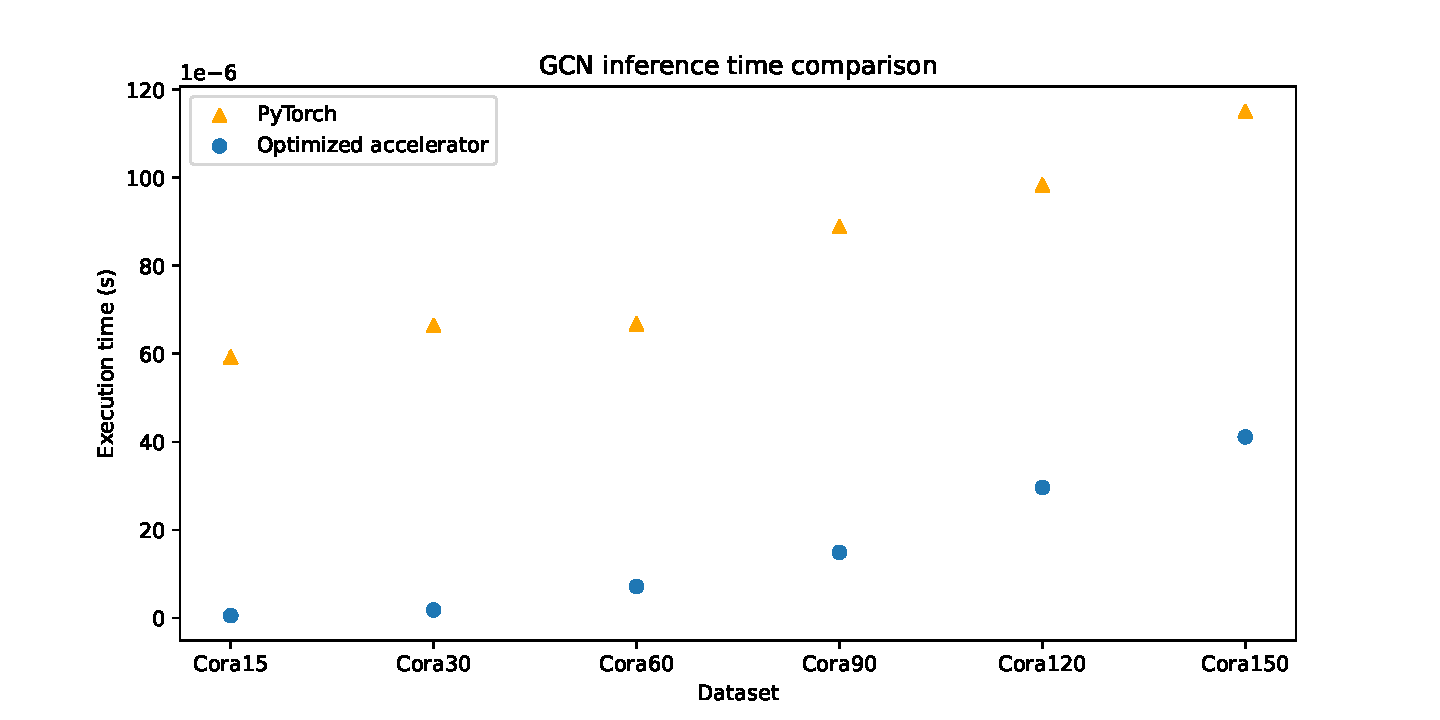
\includegraphics[height=0.4\textwidth]{Images/gcn_forward_comparison}
    \caption{GCN inference time comparison}
    \label{fig:gcn-inference-comparison}
\end{figure}

However, this behavior limits the utilization of the possibilities presented by FPGA technology, which encompass substantial parallelization potential and concurrent memory accesses.

Figure~\ref{fig:gcn-inference-comparison} and Table~\ref{tab:GCN-inference-pytorch-accelerator-comparison}, show the result of a comparative analysis between the PyTorch CPU time and the FPGA accelerator time to perform GCN inference.
All the experiments have been performed using a subset of the Cora dataset introduced in Subsection~\ref{subsec:gnn_datasets}, detailed in Table~\ref{tab:dataset-definition}.
The PyTorch times have been acquired averaging one million of execution time measurements using the PyTorch built-in benchmark API\@.

The results of this final evaluation are incredibly encouraging.
The speedup of the accelerator is not being affected by the size of the input matrices and its computation time is significantly lower with respect to the one measured on CPU with PyTorch.

The area of the accelerator, instead, is obviously affected by the sizes of the input matrices.
This because more the matrices are big, more the parallel loop iterations will be and thus the parallel processing elements.

However, the possibilities offered by the proposed toolchain are various.
It is possible to use less memory channels with a lower loop unrolling factor to still have a big positive impact on performance, but containing the accelerator area requirements.





% ##########################################################################
% CHAPTER SEVEN - CONCLUSION
% ##########################################################################

    \chapter{Conclusion and Future Developments}
    \label{ch:conclusions}%
    This thesis tackled the challenge of accelerating Graph Neural Network inference by leveraging High-Level Synthesis techniques targeting FPGAs.

An HLS-based toolchain was designed to obtain a GNN inference accelerator starting directly from PyTorch.
PyTorch stands as one of the foremost high-level frameworks for neural network implementation, extensively recognized and employed within the community, making the proposed toolchain suitable for different applications.

The results of this research significantly contribute to the field of GNN acceleration, introducing a new perspective about how it is possible to obtain hardware accelerators for GNNs even without having any hardware design knowledge.
The toolchain offers different possibilities and provides various optimization passes that can be used to fine-tune the accelerator capabilities.

Within the spectrum of optimizations made available by this toolchain, this thesis primarily delved into two key techniques: the loop unrolling technique in SODA-OPT and the parallel memory access of PandA-Bambu with an external memory of thirty-two channels.
These optimizations allowed to achieve encouraging and promising results in accelerating the inference of the GCN model analyzed.
By studying and understanding the model bottlenecks, it is possible to achieve consistent improvements.

Lastly, this study has also made substantial contribution in enhancing Torch-MLIR\@.
A new feature, the support of the constant of Tuple type, has been added and different areas of improvement have been identified, where more work would be needed to implement functionalities for the complete support of PyTorch Geometric.
Before this research, no examples were available on how to use Torch-MLIR with Graph Neural Networks, and the compatibility of PyTorch Geometric and Torch-MLIR was still an unexplored area.

\section{Future developments}
\label{sec:future-dev}%


This thesis represents a significant advancement in the field of GNN acceleration.
Nonetheless, there exist opportunities for further enhancement through the implementation of novel features.

Primarily, future works could build upon the innovative contributions of this thesis in terms of enhancing compatibility between PyTorch Geometric and Torch-MLIR\@.
PyTorch Geometric offers valuable features and pre-established classes for implementing Graph Neural Networks.
Integrating this advanced framework into the toolchain would mark another significant step forward.
This thesis identified the needed area of improvement, representing a possible starting point for these future works.

Another improvement that can be applied to the presented toolchain is the support of sparse tensors.
At the actual state, Torch-MLIR is not capable of lowering PyTorch sparse tensors to the Linalg dialect, even if it already supports them.
For this reason, some work would be needed on Torch-MLIR to implement this feature, possibly using PyTaco, which would bring a significant advantage also in the resulting accelerators, having the possibility to exploit faster computation with sparse tensors.
An additional enhancement that can be integrated into the proposed toolchain involves extending support to sparse tensors.
Currently, Torch-MLIR cannot convert PyTorch sparse tensors into the Linalg dialect, even if MLIR~\cite{9370308} already has a way to represent them~\cite{Bik_2022}.
Consequently, implementing this feature in Torch-MLIR would require dedicated efforts, producing substantial benefits in the toolchain resultant accelerators.
Even if the resulting accelerators, as discussed in Chapter~\ref{ch:chapter_six}, greatly increase performance and reduce the computational time, this enhancement would enable leveraging faster computations through the use of sparse tensors by further improving the performance of the accelerator.

In conclusion, ongoing support and dedicated efforts are consistently aimed at advancing SODA-OPT~\cite{9786533} and PandA-Bambu~\cite{9586110} through the integration of novel functionalities.
The continuous evolution of these tools represents an alternative way of progress over that the classic hardware design techniques, as the introduction of fresh SODA-OPT passes and PandA-Bambu optimizations have the potential to open novel opportunities for refining and optimizing the synthesized hardware accelerators.

%##########################################################################
%	BIBLIOGRAPHY
%##########################################################################

    \addtocontents{toc}{\vspace{2em}} % Add a gap in the Contents, for aesthetics
    \bibliography{Thesis_bibliography} % The references information are stored in the file named "Thesis_bibliography.bib"

%-------------------------------------------------------------------------
%	APPENDICES
%-------------------------------------------------------------------------

    \cleardoublepage
    \addtocontents{toc}{\vspace{2em}} % Add a gap in the Contents, for aesthetics
    \appendix

%
%    \chapter{Appendix A}
%    If you need to include an appendix to support the research in your thesis, you can place it at the end of the manuscript.
%    An appendix contains supplementary material (figures, tables, data, codes, mathematical proofs, surveys, \dots)
%    which supplement the main results contained in the previous chapters.
%
%
%    \chapter{Appendix B}
%    It may be necessary to include another appendix to better organize the presentation of supplementary material.

% LIST OF FIGURES
    \listoffigures

% LIST OF TABLES
    \listoftables

% LIST OF ALGORITHMG
    \listofalgorithms

% LIST OF LISTINGS
    \lstlistoflistings



% LIST OF SYMBOLS
% Write out the List of Symbols in this page
    \chapter*{List of Symbols} % You have to include a chapter for your list of symbols (
    \begin{table}[H]
        \centering
        \begin{tabular}{lll}
            \textbf{Notation} & \textbf{Description} \\\hline\\[-9px]
            $\mathcal{G} = (V, E)$        & The input graph for the GNN  \\[2px]
            $V$ & Set of vertices of the graph \\[2px]
            $E$ & Set of edges of the graph \\[2px]
            $\mathcal{N}(v)$ & Set of neighbors of vertex $v$ \\[2px]
            $A \in \mathbb{R}^{N \times N}$        & Adjacency matrix of $\mathcal{G}$ ($N$ : number of nodes)  \\[2px]
            $\tilde{D}$ & Degree matrix of the graph \\[2px]
            $W^{(l)}$ & Weight matrix of the neural network ($l$ : layer) \\[2px]
            $H^{(l)}$ & Input node features matrix ($l$ : layer) \\[2px]
            $h_v$ & Node representation of node $v$ \\[2px]
            $\epsilon$ & Learnable parameter or fixed scalar \\[2px]
            $I$ & Identity matrix \\[2px]

        \end{tabular}\label{tab:symbols_table}
    \end{table}

% ACKNOWLEDGEMENTS
    \chapter*{Acknowledgements}
    Acknowledgements here...

    \cleardoublepage

\end{document}
